\documentclass[12pt]{article}
\usepackage[margin=1in]{geometry} 		% defines page margin
\usepackage{knitting} 				% defines \chart and \textknit
\usepackage{titling} 				% title page
\usepackage{graphicx,xspace, scrextend}	% defines space control stuff
\usepackage{tabularx, array, colortbl}	% defines tables
\usepackage{multicol} 				% defines columns
\usepackage{multirow} 				% defines multirows, combined cells in tables
\usepackage{framed} 				% defines boxes for notes and written directions
\usepackage[x11names]{xcolor} 		% extends color library
\pdfmapfile{+knitfont.map}

\renewcommand{\arraystretch}{2}

\newcolumntype{L}[1]{>{\arraybackslash}p{#1}}
\newcolumntype{C}[1]{>{\centering\arraybackslash}p{#1}}

% length parameters
\setlength{\parindent}{0pt} % disables indentation for paragraphs
\setlength{\columnsep}{0.7cm} % column separation in multicol environment

% color parameters
\colorlet{framecolor}{black}
\colorlet{shadecolor}{LemonChiffon1}
\colorlet{highlight}{yellow}

% custom commands
\newcommand{\comment}[1]{} % allows for multiline comments that LaTeX will ignore

\newcommand{\vocab}[1]{\emph{\textbf{#1}}} % format for highlighting definitions of stitches, vocabulary terms
\newcommand{\rowDir}[1]{\hspace{-2em} \textbf{#1:}} % indent for written instructions within paragraphs
\newcommand{\spine}[1]{\colorbox{highlight}{#1}} % highlights spine stitches
\newcommand{\increase}[1]{(\emph{+#1 
	\ifnum#1=1{st}\else{sts}\fi})}
\newcommand{\decrease}[1]{(\emph{$-$#1
	\ifnum#1=1{st}\else{sts}\fi})}

\renewcommand{\rm}{\emph{rm}} % remove marker
\renewcommand{\pm}{\emph{pm}} % place marker

% thick horizontal line
\makeatletter \newcommand{\thickhline}{
    \noalign {\ifnum 0=`}\fi \hrule height 1.5pt
    \futurelet \reserved@a \@xhline
}
\makeatother

% custom environments
\newenvironment{frnote}
    {% framed environment for pattern notes
    	\setlength{\FrameRule}{1.5pt}
    	\def\FrameCommand{\fboxrule=\FrameRule\fboxsep=\FrameSep \fcolorbox{framecolor}{shadecolor}}
    	\MakeFramed {\FrameRestore}}
    {\setlength{\FrameRule}{1pt}
	\endMakeFramed}

\newenvironment{frdirection}
    {% framed environment for written directions
	\def\FrameCommand{\fboxrule=\FrameRule\fboxsep=\FrameSep \fbox}
   	\MakeFramed {\advance\hsize-\width \FrameRestore}
    	\addmargin[1.5cm]{0pt}}
    {\endaddmargin
	\endMakeFramed}

\newenvironment{unframed}
    {% unframed environment for written directions
	\begin{addmargin}[1.5cm]{0pt}}
    {\vspace{1em}
	\end{addmargin}}

\title{Mitered Nova}
\author{Shanel Wu (Piper Nell)}

\begin{document}
\begin{titlingpage}

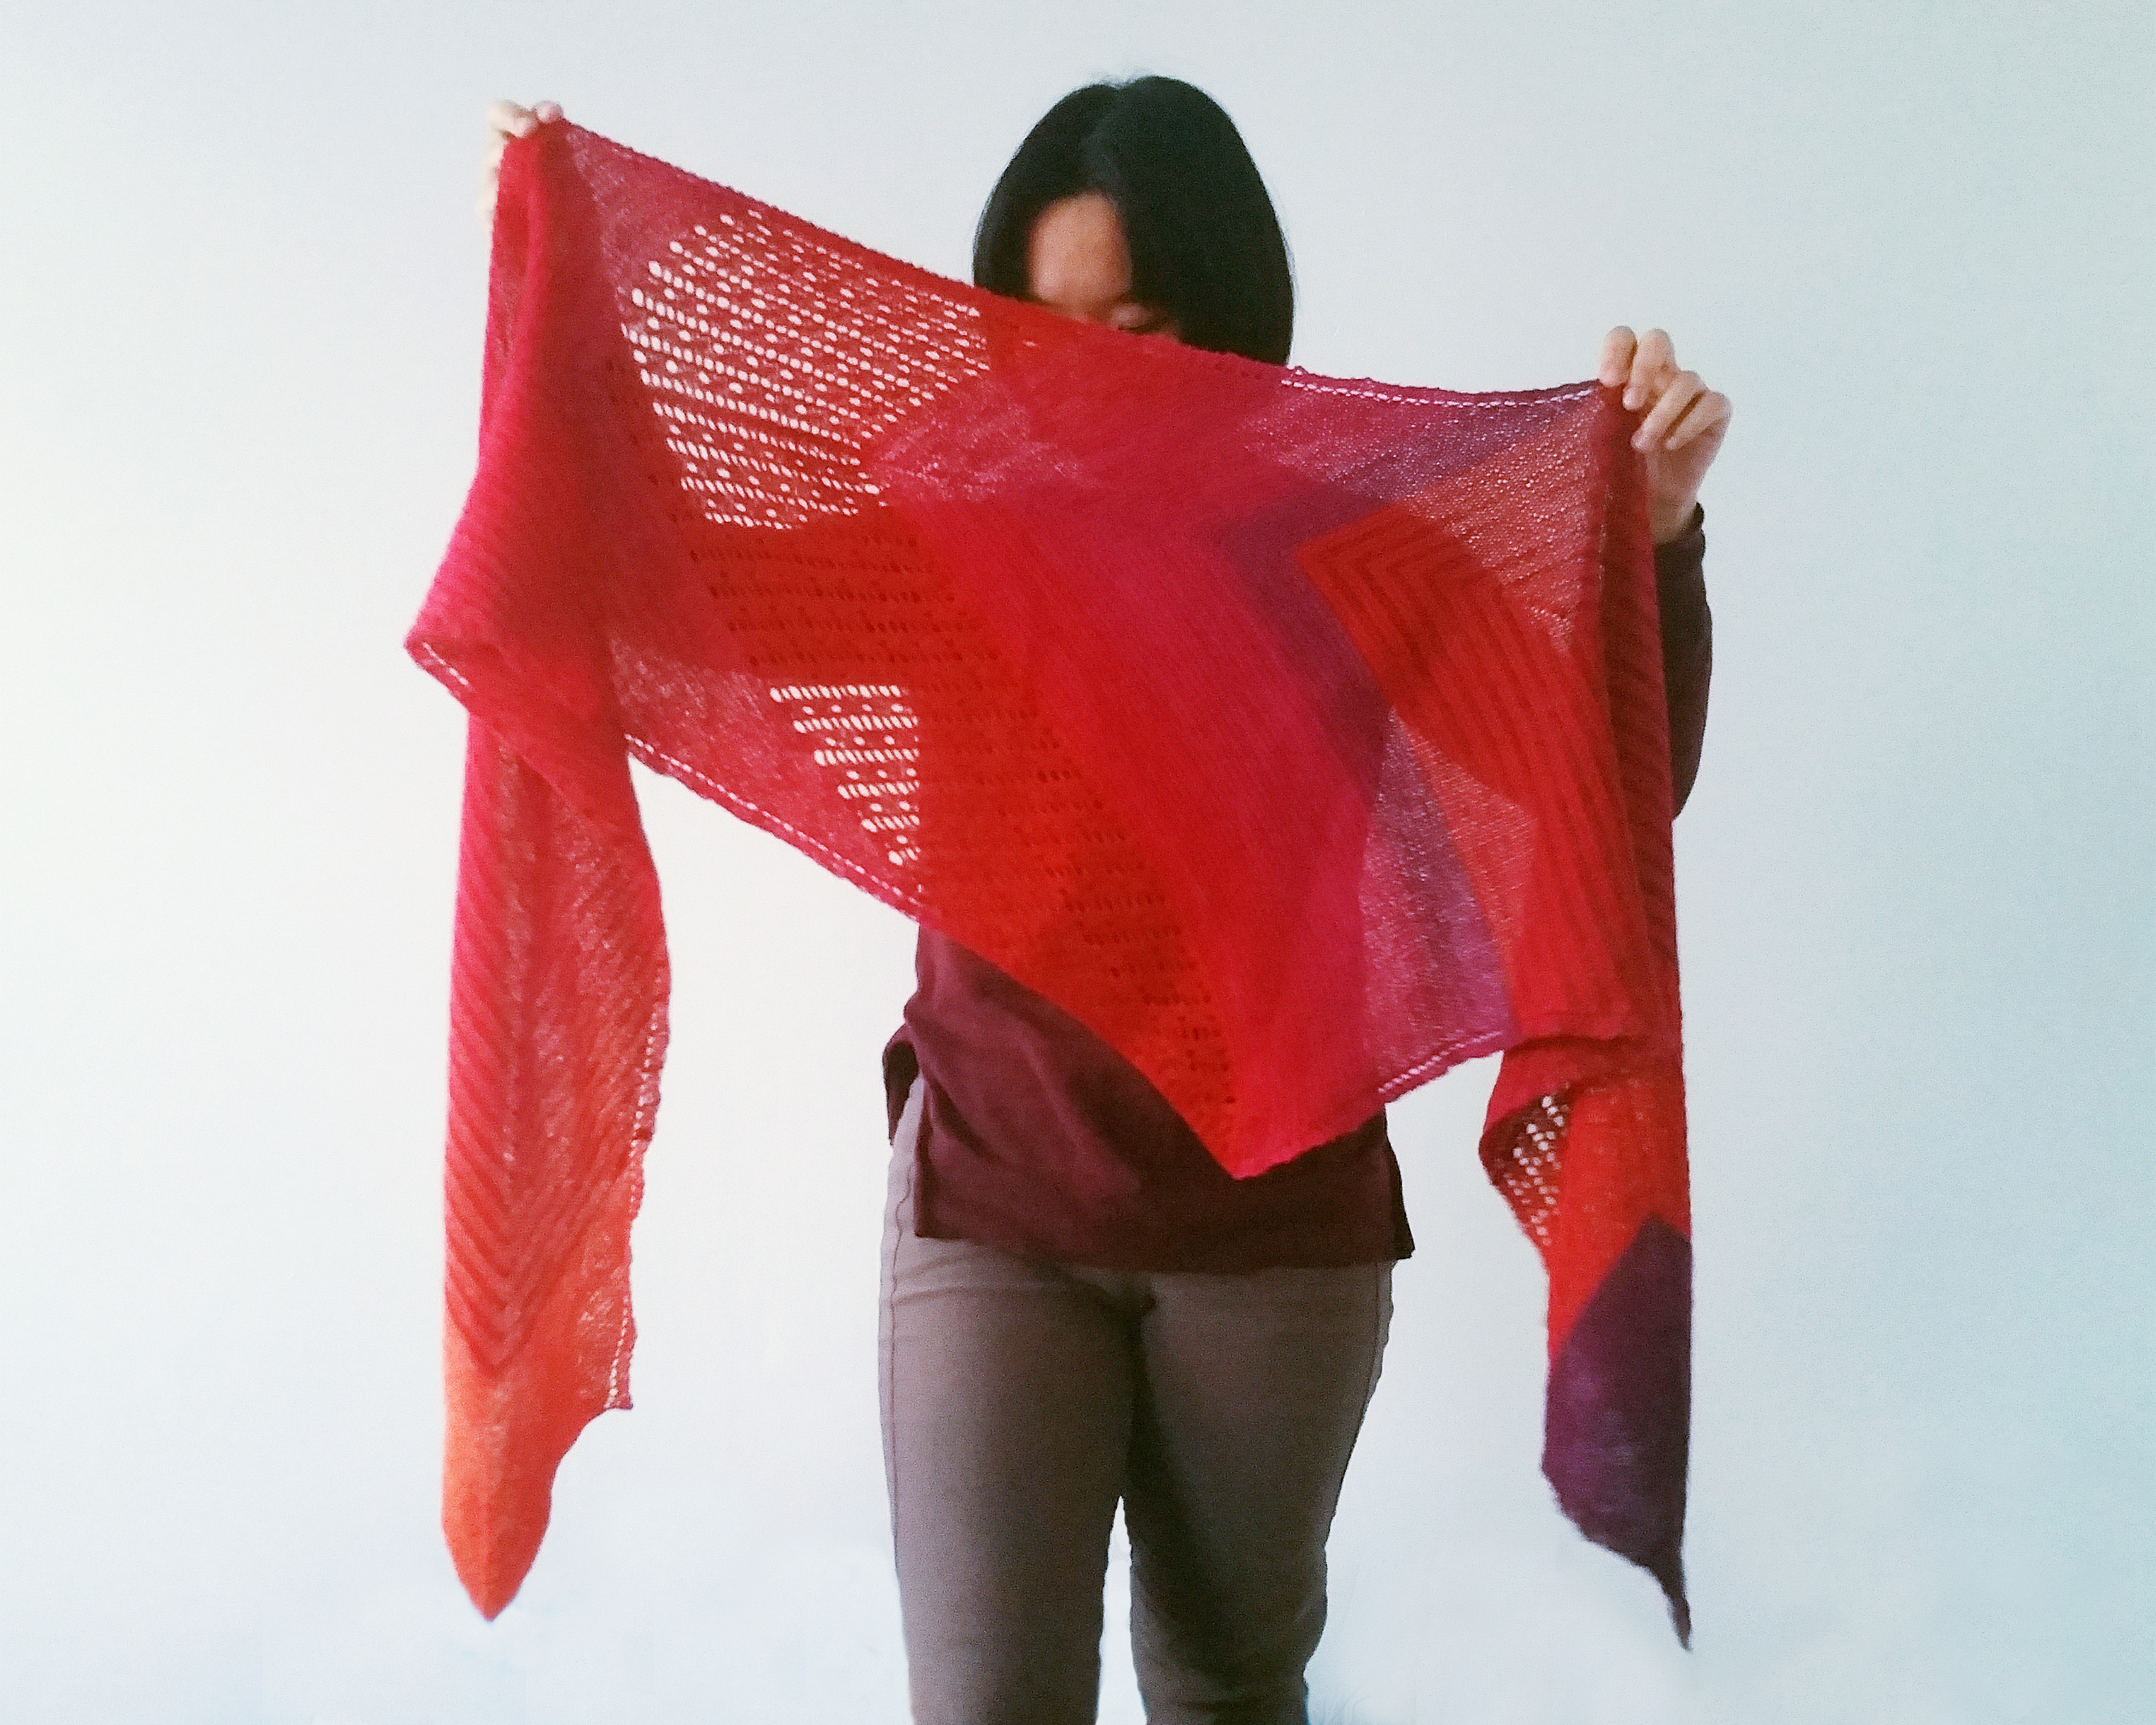
\includegraphics[width=\textwidth]{LW-holdFront}

\begin{multicols}{2}

\section*{\thetitle}
\subsubsection*{\theauthor}

Starts like a mitered square, ends like a mitered square---but something stellar happens in between! You cast on at a short end and knit this shawl sideways with a central spine throughout. As you progress from one tip to the other, the shawl expands like a star in the twilight of its life, then explodes in a nova of lace. Suddenly, the shawl contracts, gradually becoming narrower until nothing is left.

\vspace{-1em}
\subsubsection*{Materials}

You'll need two colors (C1 and C2) and a long (at least 32") circular needle. \\ Yardage, sample gauge, and recommended needle sizes are in the table that follows. Gauge is not important, but may affect yarn consumption and final size of the piece.

\vspace{-1em}
\subsubsection*{Notions}
\begin{itemize}
\item Tapestry needle \vspace{-1em}
\item Removable stitch markers (optional)
\end{itemize}

\vspace{-2em}
\subsubsection*{Yarn Choice}

I designed the shawl to show off a gradient C1, with any C2 suited to your taste. The laceweight weight sample is knit with C1 in Freia Ombre Lace in ``Flare", a gradient that shifts through multiple warm hues, and with C2 in Knit Picks Gloss Lace in ``Fiesta", a solid color which matches one of the hues in the gradient. The fingering weight sample is knit with C1 in Wee Chickadee Woolery's gradient yarn, a light-to-dark tonal gradient of warm brown, and C2 is Wee Chickadee's sock base, a speckled yarn that complements the earthy brown C1.

\vspace{-1em}
\subsubsection*{Techniques and Reading}

This pattern is for intermediate knitters with some lace experience, so knowledge of k2tog, ssk, and yarn overs is assumed. Instructions included for double increases and decreases, striping with carrying yarn up the side, and right- and left-twist stitches (i.e. 1x1 cables). Some experience with mitered square construction is recommended.

\vspace{1em}
One set of directions is given for both versions of the shawl, lace weight and fingering weight. Repeat and stitch counts differ by yarn weight and are given in the format \mbox{\vocab{lace(fingering)}. [e.g. knit 45(35) sts]} 

You may find it helpful to count the repeats by counting garter ridges.

\end{multicols}

\vfill

% materials table w/ yardage and needle size for two versions
\begin{tabular}{ | C{0.15\linewidth}  C{0.4\linewidth}  C{0.4\linewidth} |}
\thickhline \rowcolor{shadecolor}
{} 			&\textbf{Lace weight} 	& \textbf{Fingering weight} \\ \thickhline
\textbf{Yardage}	& C1: 75g/645y, C2: 50g/400y		& C1: 100g/420y, C2: 100g/420y \\
\textbf{Gauge}	& {26 st x 46 rows/4"(10cm)}	& {23 st x 40 rows/4"(10cm)} \\ 
\textbf{Needle} \mbox{(32" or longer)}	& US3 (2.75mm)		& US5 (3.75mm) \\ \hline
\end{tabular}

\vfill

\begin{center}
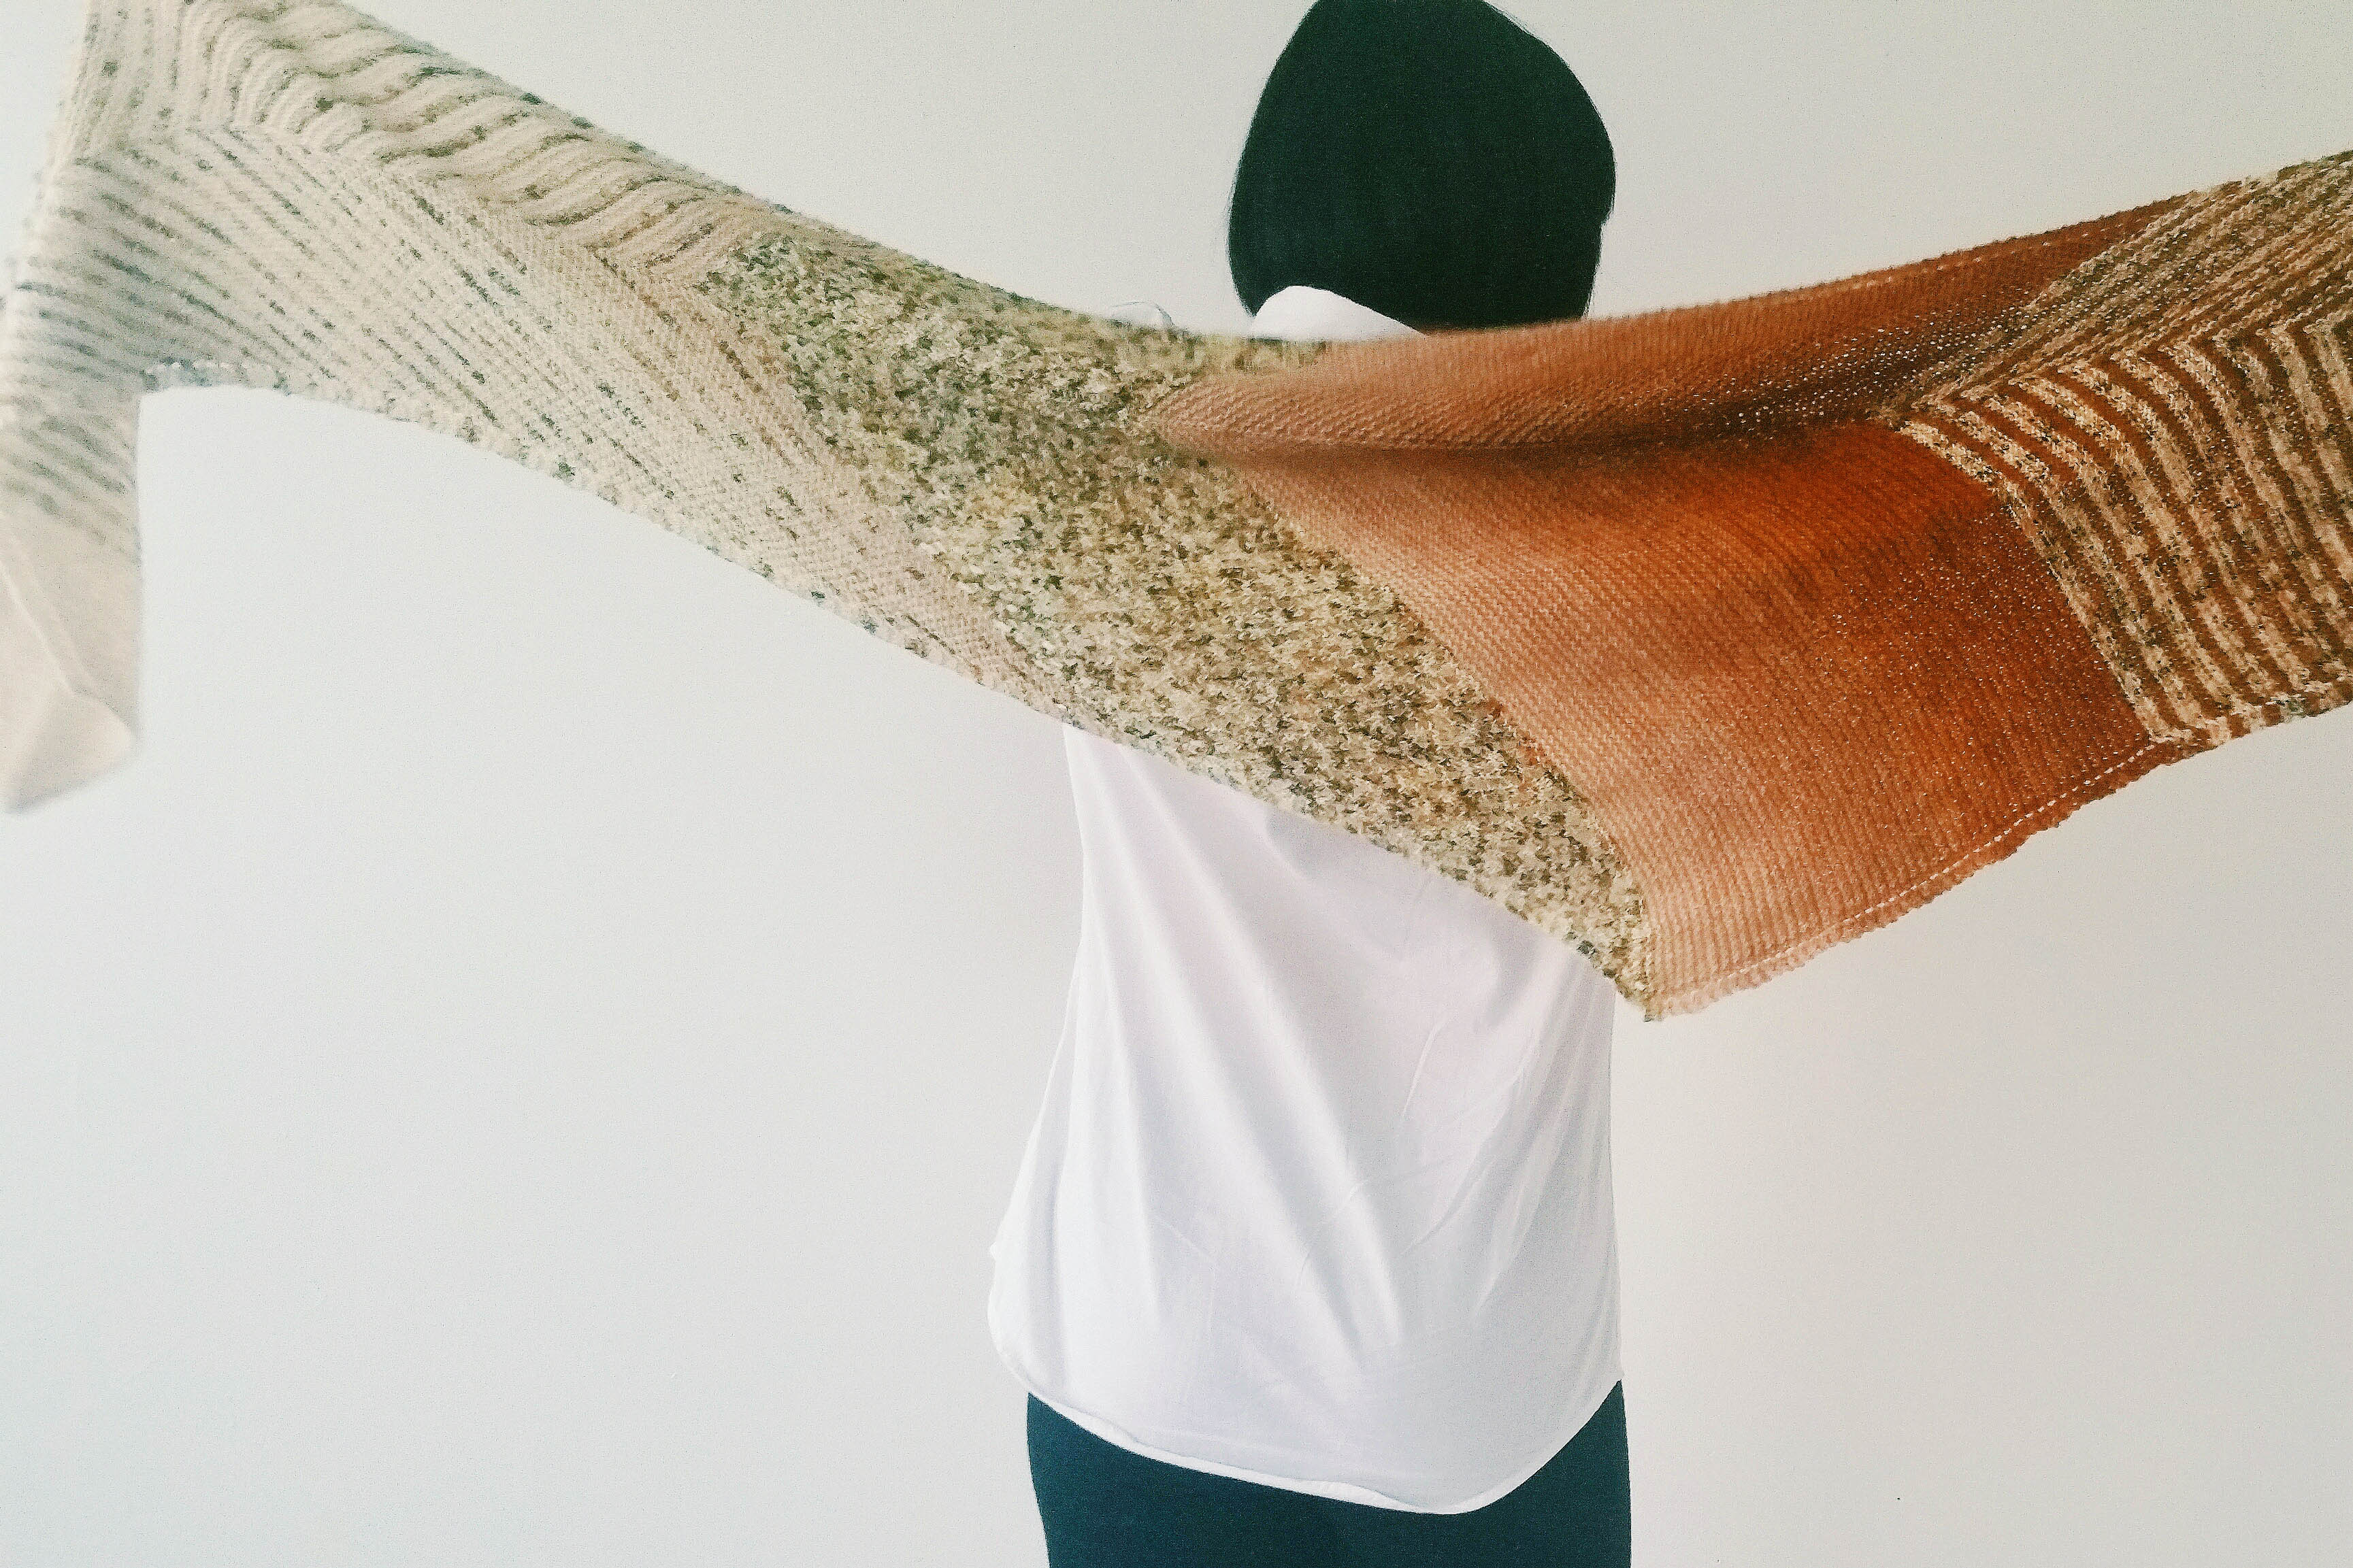
\includegraphics[width = 6.5in]{FW-spread-small} \end{center}
\end{titlingpage}

%%%%%%%%%%%%%%%%%%%%%%%%%%%%%%%%%%%%%%%%
\subsection*{Pattern Key}

Pattern repeats will be indicated with thick borders (chart) or asterisks \textbf{*[stitches]*} (written). Spine stitches will be \spine{highlighted}. All odd-numbered rows will be on the right side of the work (RS) and all even-numbered rows will be on the wrong side (WS).
\vspace{-1em}
\begin{center}
\begin{tabular}{| C{0.15\linewidth}  C{0.2\linewidth}  p{0.6\linewidth} | }
\thickhline \rowcolor{shadecolor} 
\textbf{Chart}	& \textbf{Written}	& \textbf{Name \& Description} \\ \thickhline
\chart{-}	& k (RS); p (WS)	&  knit (RS); purl (WS)	\\
\chart{=} 	& p (RS); k (WS)	& purl  (RS); knit (WS) \\
N/A		& s1 wyib		& slip one stitch with yarn in back \\
\chart{kK} 	& r2t		& right twist or right mini-cable \emph{(See appendices.)}\\
\chart{Kk}	& l2t		& left twist or left mini-cable \emph{(See appendices.)} \\  
\multicolumn{3}{| c |}{\cellcolor{shadecolor}\textbf{increases}} \\ 
\chart{O} 	& yo		& yarn-over  \\
\chart{v}	& kfb		& \textbf{knit front back:} knit stitch through front loop, then in the same stitch, knit through the back loop; single increase		\\
\chart{w}	& kyok	& \textbf{knit yarn-over knit:} in a single stitch, knit, yarn over, then knit again; double increase		\\ 
\multicolumn{3}{| c |}{\cellcolor{shadecolor} \textbf{decreases}} \\ \
\chart{>}	& k2tog 	& \textbf{knit 2 together:} single decrease, right-leaning \\
\chart{<}	& ssk		& \textbf{slip slip knit:} single decrease, left-leaning \\
\chart{A} 	& cdd		& \textbf{central double-decrease:} slip two stitches as if to k2tog, k next stitch, pass 2 slipped st over \\
\chart{R}	& k3tog 	& \textbf{knit 3 together:} double decrease, right-leaning \\
\chart{L}	& sssk		& \textbf{slip slip slip knit:} slip 3 knitwise individually, k3tog through back loop; double decrease, left-leaning \\
\hline
\end{tabular}
\end{center}

%%%%%%%%%%%%%%%%%%%%%%%%%%%%%%%%%%%%%%%%
\newpage
\section*{Section 1: Steady State}

\begin{unframed}
\rowDir{Cast On} With C1, CO 91 (71) stitches using the long-tail cast on. \\ The middle stitch, the 46th (36th) stitch, will be referred to as the \vocab{spine stitch} or the \vocab{spine} and will be \spine{highlighted} when appropriate. On every RS row, the spine stitch will be the center stitch in a centered double-decrease (cdd). On every WS row, the spine stitch will be purled.
 
\rowDir{Set-up row} (WS) k 45 (35) sts, \spine{p1}, k to end. 
\end{unframed}

Next, work 25 (20) repeats of Rows 1-2 as follows, for a total of 50 (40) rows. Each repeat forms a \vocab{straight ridge} in garter stitch.

\begin{frdirection}
\rowDir{Row 1} (RS) k3, yo, k to 1 st before spine, \spine{cdd},  k to 3 sts before end, yo, k3.

\rowDir{Row 2} (WS) k to spine, \spine{p1}, k to end.
\end{frdirection}

You should end Section 1 with the same number of stitches as you started, 91 (71) sts.

\begin{frnote}
\textbf{Shaping:}  Shaping (increases and decreases) is worked on WS rows into the yo of the preceding RS row. See Appendix C for tips on modifying the shawl size.

\textbf{Edge Modification:} If your edges in garter stitch tend to be loose, try slipping the first or last stitch of every row.

\textbf{Stitch markers:} Some test knitters found that marking the spine with a stitch marker helped them read their work. Experiment with different marker placements to see what helps you!
\end{frnote}

%%%%%%%%%%%%%%%%%%%%%%%%%%%%%%%%%%%%%%%%
\section*{Section 2: Expanding Stripes}
\begin{unframed}
\rowDir{Set-up stripe (6 rows)} Switch to C2 and work one \textbf{straight ridge}. Then switch back to C1, carrying C2 up the edge, and work two more \textbf{straight ridges}. 
\end{unframed}

Next, work 30 (20) repeats of Rows 1-6 as follows. Each 6-row repeat forms one \vocab{increase stripe}, consisting of one \textbf{increase ridge} in C2 (Rows 1-2) then two \textbf{straight ridges} in C1, increasing by 1 st per repeat. 

\begin{frdirection}
\rowDir{Row 1} (C2) k3, yo, k to 1 st before spine, \spine{cdd}, k to 3 sts before end, yo, k3.

\rowDir{Row 2} (C2) k to spine, \spine{p1}, k to 4 sts from end, kfb, k3. \increase{1}
\\ (\emph{Rows 1-2 form an \textbf{increase ridge}})

\rowDir{Row 3} (C1) Repeat Row 1.

\rowDir{Row 4} (C1) k to spine, \spine{p1}, k to end.

\rowDir{Row 5 \& 6} (C1) Repeat Rows 3 \& 4.
\end{frdirection}

At the end of Section 2, you should have 121 (91) sts. 

%%%%%%%%%%%%%%%%%%%%%%%%%%%%%%%%%%%%%%%%
\newpage
\section*{Section 3: Lace Nova}
Lace instructions are both written and charted according to the pattern key. The main lace motif is a 5-stitch, 6-row repeat where all wrong side sts (minus edge stitches) are purled. WS rows after Row 2 are omitted in the written instructions. Increases are worked into yo of previous row. Each repeat of \textbf{Chart A} increases by 5 sts.
\vspace{1em}
\begin{unframed} \rowDir{Set-up (2 rows)} Break C1, switch to C2, and work one \textbf{straight ridge} as follows: \end{unframed}
\vspace{-2em}
\begin{frdirection}
\rowDir{Row 1} (RS) k3, yo, k to 1 st before spine, \spine{cdd},  k to 3 sts from end, yo, k3.

\rowDir{Row 2} (WS) k to spine, \spine{p1}, k to end.
\end{frdirection}

Next, work 8 (8) repeats of \textbf{Chart A}. \vspace{-1em}

\subsection*{Chart A}

\chart{
\rnleft ===\!\overline{-----}\!--\spine{-}--\!\overline*{-----}\!-------w===
---\!OLO--\!O-\spine{A}-O\!--ORO\!--ORO--O--- \rnright
\rnleft ===\!-----\!--\spine{-}--\!-----\!-----v===
---\!O<Kk-\!O-\spine{A}-O\!-kK>O\!-kK>-O--- \rnright
\rnleft ===\!-----\!--\spine{-}--\!-----\!----v===
---\!\underline*{O<-Kk}\!O-\spine{A}-O\!\underline*{kK->O}\!kK->O---		\rnright
}

\subsection*{Chart A (written)}
\begin{unframed} 
\rowDir{Row 1} k3, yo, k2tog, k1, r2t, \textbf{*[yo, k2tog, k1, r2t]*} to 2 sts before spine, \\ yo, k1, \spine{cdd}, k1, yo, \textbf{*[l2t, k1, ssk, yo]*} to 3 sts from end, k3

\rowDir{Row 2} k3, p to 4 sts from end, kfb, k3 \increase{1}

\rowDir{Row 3} k3, yo, k1, k2tog, r2t, k1, \textbf{*[yo, k2tog, r2t, k1]*} to 2 sts before spine, \\ yo, k1, \spine{cdd}, k1, yo, \textbf{*[k1, l2t, ssk, yo]*} to 3 sts from end, k3

\rowDir{Row 4} Repeat Row 2. \increase{1}

\rowDir{Row 5} k3, yo, k2, yo, k3tog, yo, k2, \textbf{*[yo, k3tog, yo, k2]*} to 2 sts before spine, \\ yo, k1, \spine{cdd}, k1, yo, \textbf{*[k2, yo, sssk, yo]*} to 3 sts from end, k3 \increase{1}

\rowDir{Row 6} k3, p to 4 sts from end, kyok, k3 \increase{2}
\end{unframed}

After the last lace repeat, work one more \textbf{straight ridge} before moving onto the next section. At the end of Section 3, you should have 161 (131) sts.

%%%%%%%%%%%%%%%%%%%%%%%%%%%%%%%%%%%%%%%%
\newpage
\section*{Section 4: Contracting}
Break C2 and switch to C1. Work 40 (30) repeats of Rows 1-2 as follows. Each repeat decreases 1 st and forms a \vocab{decrease ridge}.

\begin{frdirection}
\rowDir{Row 1} k3, yo, k to 1 st before spine, \spine{cdd}, k to 3 sts from end, yo, k3.

\rowDir{Row 2} k to spine, \spine{p1}, k to 6 sts from end, k2tog, k4. \decrease{1}
\end{frdirection}

At the end of Section 4, you should have 121 (101) sts on your needles.


%%%%%%%%%%%%%%%%%%%%%%%%%%%%%%%%%%%%%%%%
\section*{Section 5: Contracting Stripes}
Rejoin C2. Work 15 (15) repeats of Rows 1-6 as follows, decreasing while striping C1 and C2. Each 6-row repeat forms one \vocab{decrease stripe}, consisting of two \textbf{decrease ridges} in C2 followed by one \textbf{straight ridge} in C1, decreasing by 2 sts per repeat.

\begin{frdirection}
\rowDir{Row 1} (C2) k3, yo, k to 1 st before spine, \spine{cdd}, k to 3 sts from end, yo, k3.

\rowDir{Row 2} (C2) k to spine, \spine{p1}, k to 6 sts from end, k2tog, k4. \decrease{1}

\rowDir{Rows 3 \& 4} (C2) Repeat Rows 1 \& 2. \decrease{1}

\rowDir{Row 5} (C1) Repeat Row 1.

\rowDir{Row 6} (C1) k to spine, \spine{p1}, k to end.
\end{frdirection}

At the end of Section 5, you should have your original stitch count, 91 (71) sts.

\vfill
\begin{center}
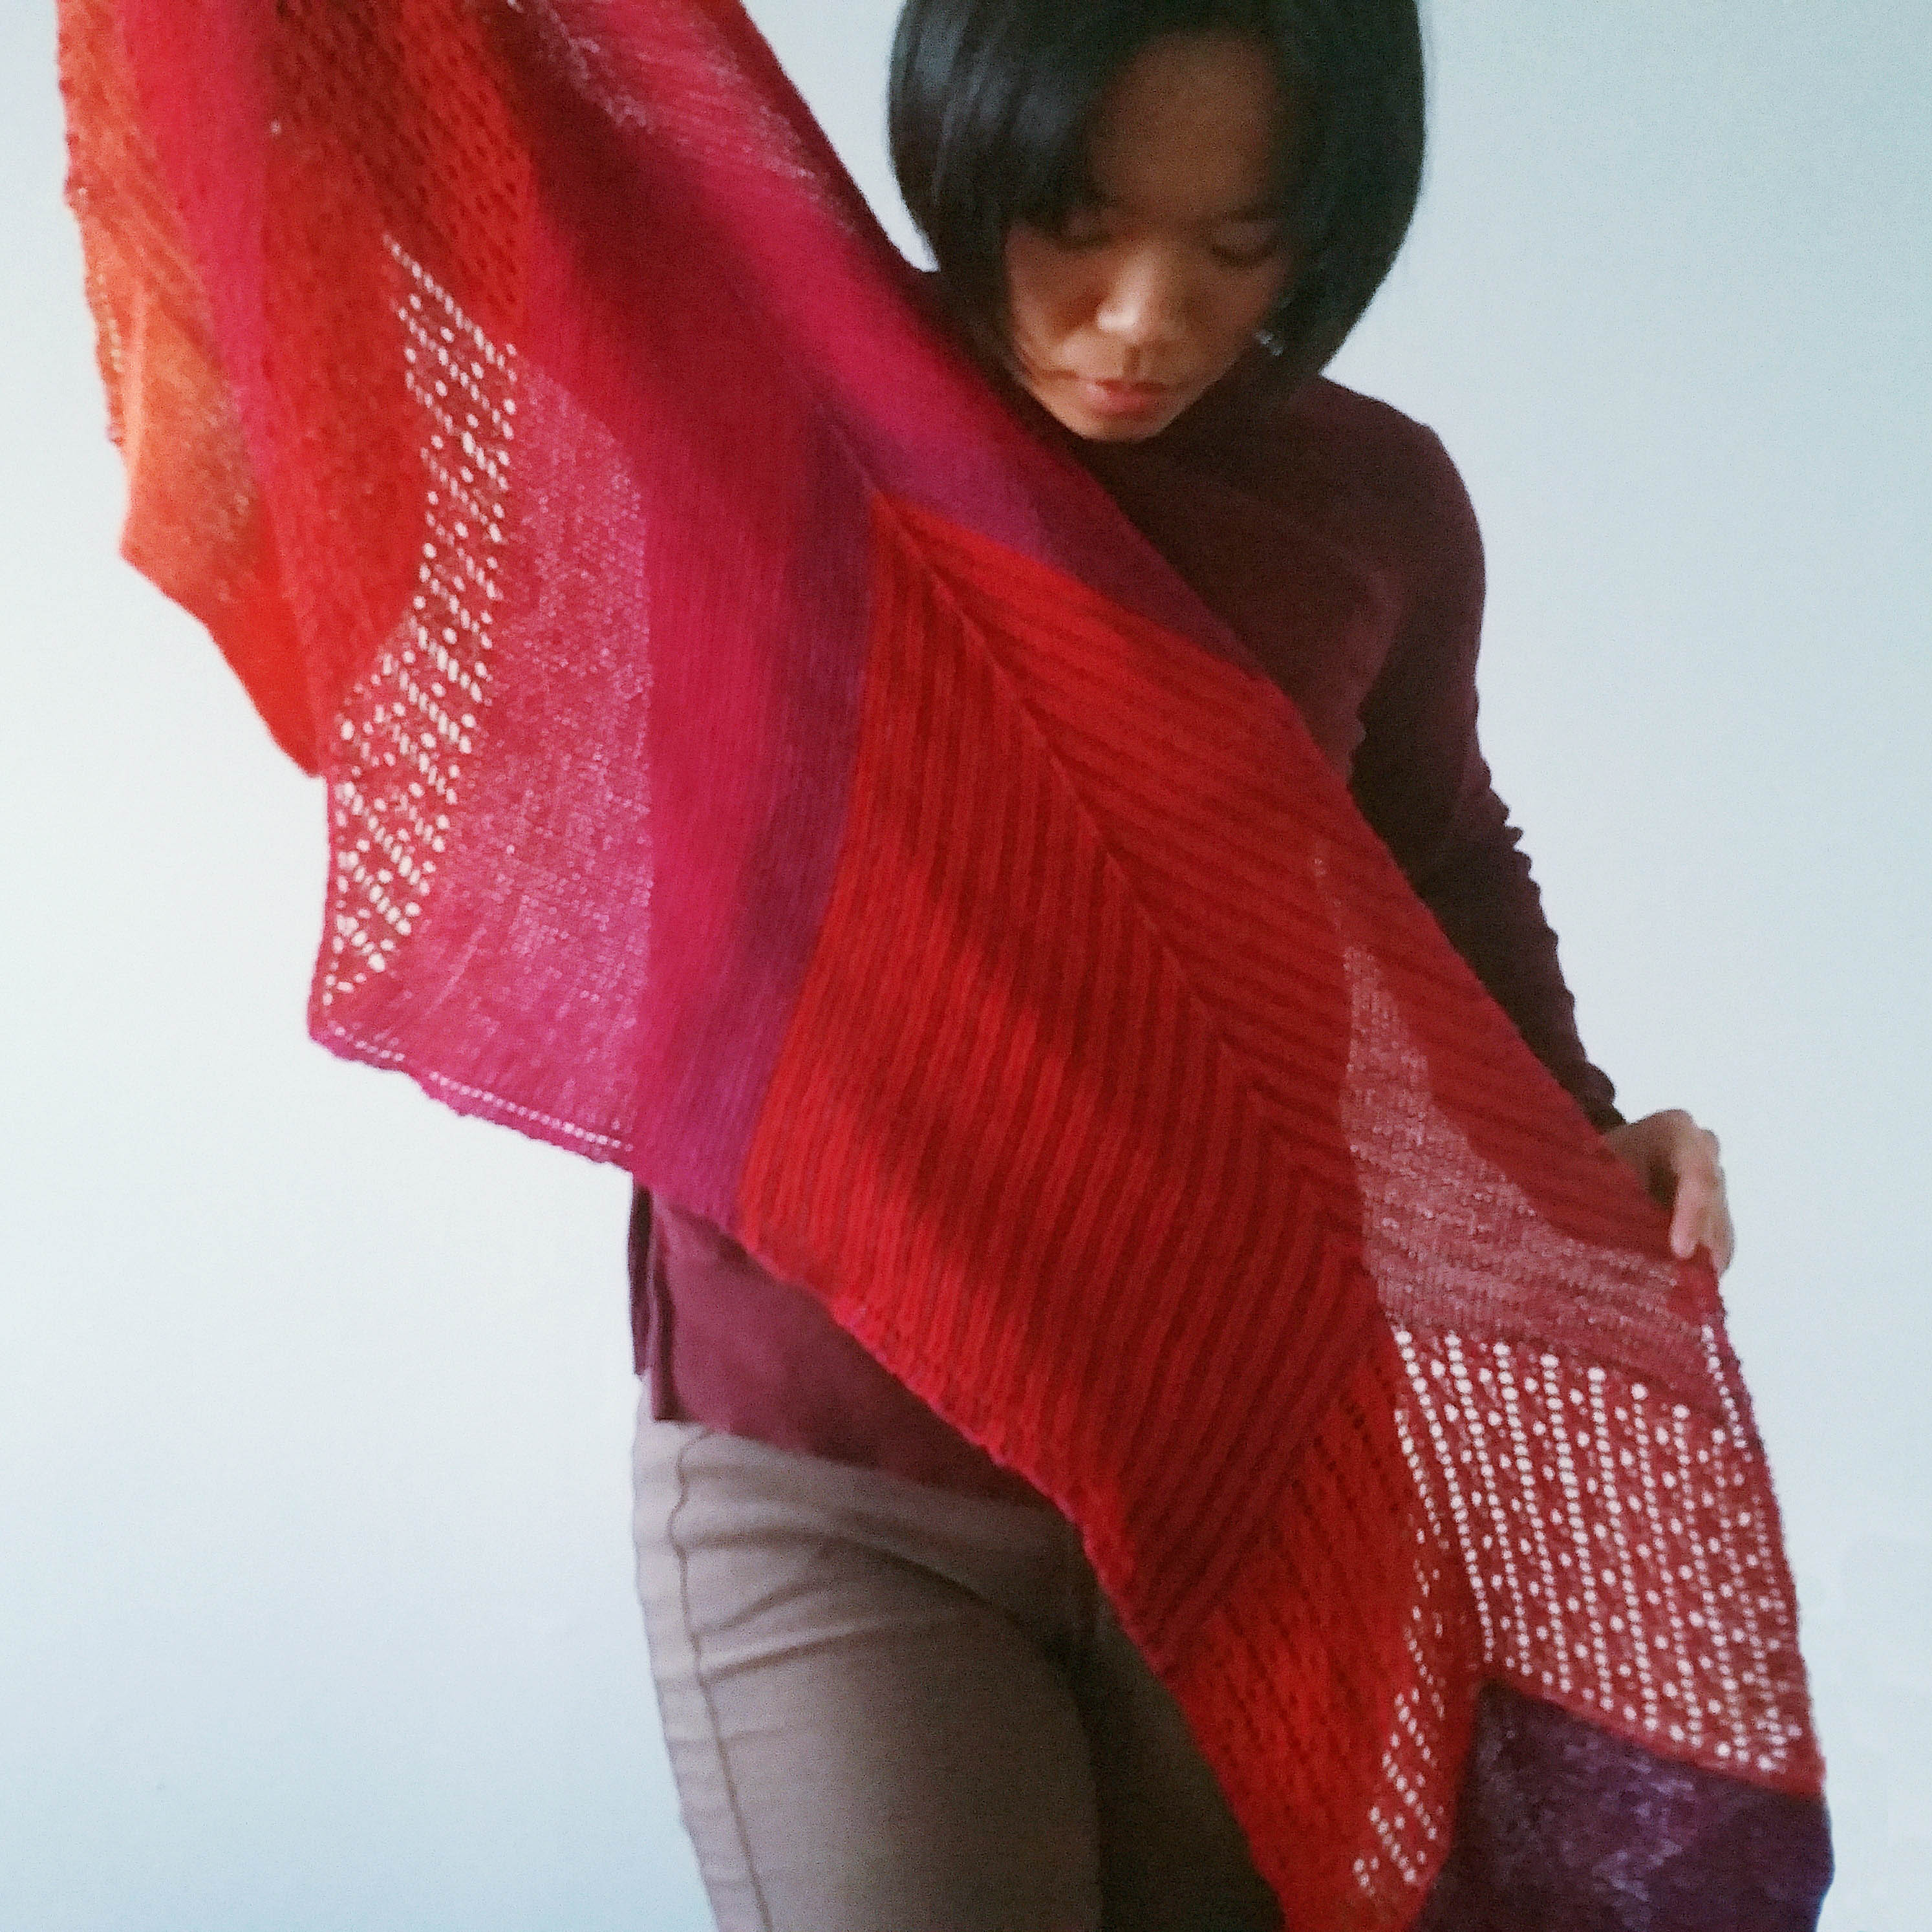
\includegraphics[height=3.2in]{LW-holdDetail-small} \hfill
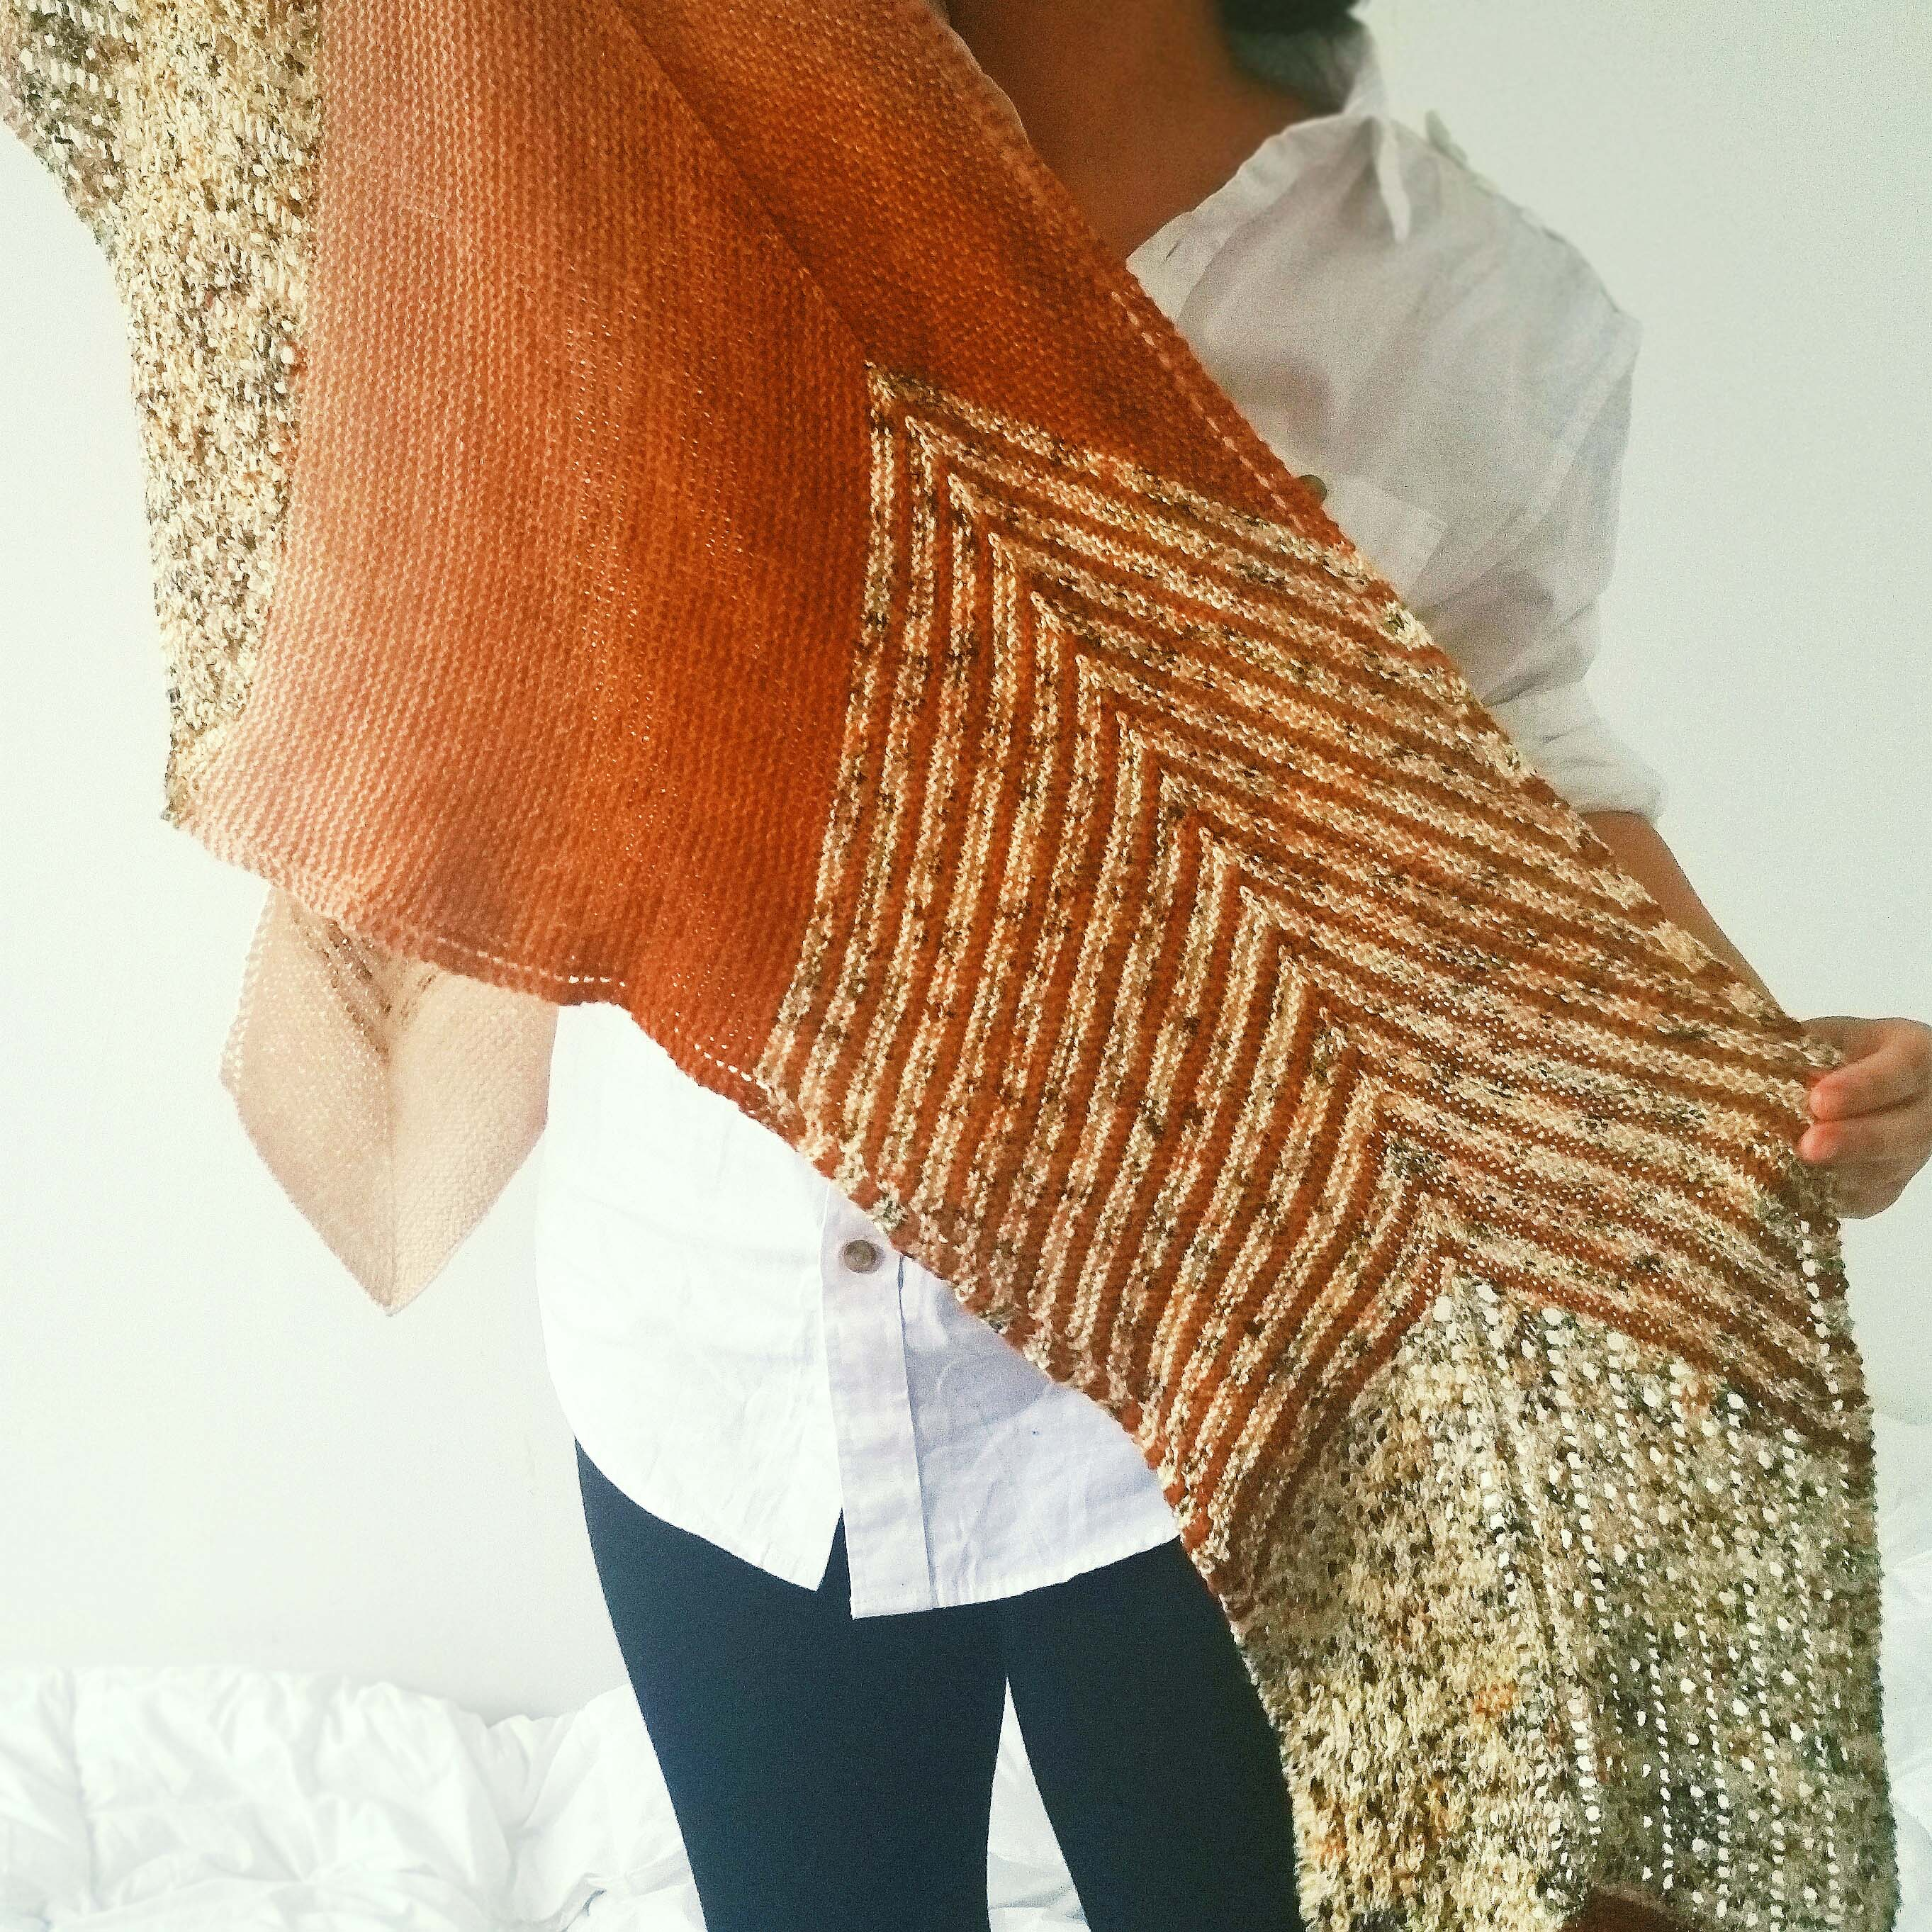
\includegraphics[height=3.2in]{FW-holdDetail-small}
\end{center}

%%%%%%%%%%%%%%%%%%%%%%%%%%%%%%%%%%%%%%%%
\newpage
\section*{Section 6: Lace Steady State}
\begin{unframed} \rowDir{Set-up (2 rows)} Break C1, switch to C2, and work one \textbf{straight ridge}. \end{unframed}
\vspace{-2em}
\begin{frdirection}
\rowDir{Row 1} (RS) k3, yo, k to 1 st before spine, \spine{cdd},  k to 3 sts before end, yo, k3.

\rowDir{Row 2} (WS) k to spine, \spine{p1}, k to end.
\end{frdirection}

Next, work 8 (10) repeats of \textbf{Chart B}. 
\subsection*{Chart B}

\chart{
\rnleft ===\!\overline{-----}\!--\spine{-}--\!\overline*{-----}\!=== 
---\!OLO--\!O-\spine{A}-O\!--ORO\!--- \rnright
\rnleft ===\!-----\!--\spine{-}--\!-----\!===
---\!O<Kk-\!O-\spine{A}-O\!-kK>O\!--- \rnright
\rnleft ===\!-----\!--\spine{-}--\!-----\!===
---\!\underline*{O<-Kk}\!O-\spine{A}-O\!\underline*{kK->O}\!--- \rnright
}

\subsection*{Chart B (written)}

\begin{unframed}
\rowDir{Row 1} k3, \textbf{*[yo, k2tog, k1, r2t]*} to 2 sts before spine, yo, k1, \spine{cdd}, k1, yo, \textbf{*[l2t, k1, ssk, yo*]} to 3 sts from end, k3 

\rowDir{Row 2} k3, p to 3 sts from end, k3 \emph{(all WS rows are identical to Row 2)}

\rowDir{Row 3} k3, \textbf{*[yo, k2tog, r2t, k1]*} to 2 sts before spine, yo, k1, \spine{cdd}, k1, yo, \textbf{*[k1, l2t, ssk, yo]*} to 3 sts from end, k3

\rowDir{Row 5} k3, \textbf{*[yo, k3tog, yo, k2]*} to 2 sts before spine, yo, k1, \spine{cdd}, k1, yo, \textbf{*[k2, yo, sssk, yo]*} to 3 sts from end, k3
\end{unframed}

After the last lace repeat, work one more \textbf{straight ridge} before moving on. You should end Section 6 with the same number of stitches as you started, 91 (71) sts.

%%%%%%%%%%%%%%%%%%%%%%%%%%%%%%%%%%%%%%%%
\begin{multicols}{2}
\section*{Section 7: Mitered Square}

Break C2 and switch to C1 for this last section. Work a mitered square by repeating the following two rows:

\begin{unframed}
\rowDir{Row 1} (RS) slip 1 with yarn in back (\textbf{s1 wyib}), k to 1 before spine, \spine{cdd}, k to end

\rowDir{Row 2} (WS) s1 wyib, k to spine, \spine{p1}, k to end
\end{unframed}

Each repeat decreases by 2 sts. Repeat Rows 1 and 2 until 5 sts are left at the end of a WS row. 

Work the last 3 rows as follows:

\begin{unframed}
\rowDir{Row 1} (RS) s1 wyib, cdd, k1 (3 sts)

\rowDir{Row 2} (WS) k1, p1, k1 (3 sts)

\rowDir{Row 3} (RS) cdd (1 st)
\end{unframed}

Break yarn, leaving a 6 inch tail. Pull the loop of the last stitch through to finish. 

\begin{frnote}
\textbf{Finishing:} Block the piece, weave in all ends, and enjoy your new shawl! I would recommend blocking wires for the edges. I also suggest pinning down the spine as you block to help shape the shawl.
\end{frnote}
\end{multicols}

\newpage
%%%%%%%%%%%%%%%%%%%%%%%%%%%%%%%%%%%%%%%%

\section*{Appendix A: Carrying Yarn Up the Side of Your Work}

\begin{multicols}{2}
While working the striped sections (2 and 5) of the Mitered Nova, you'll be working with one color at a time and carrying the other color up the side. The technique in this tutorial is based on my personal preference.

\subsection*{Adding the Contrast Color}
% Step 1: drop old color and add in new color
\begin{enumerate}
\item At the start of a RS row, drop main color (MC) working yarn. Add in contrast color (CC) for stripes by working the first stitch of the row in CC. \emph{Tip: hold the tail of CC with MC with your non-tensioning hand.}

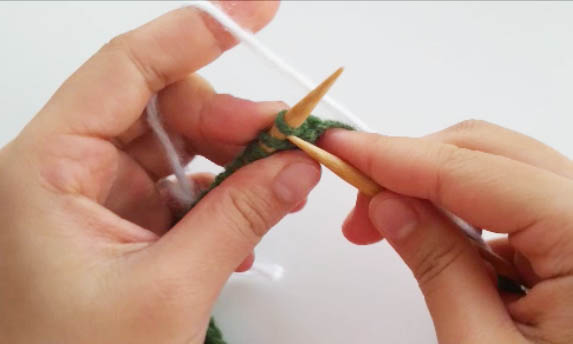
\includegraphics[width=2.5in]{addCC.jpg}

\item Work the rest of the row in the new color, turn the piece, then work a WS row. You should have two yarns attached to your work, as shown below. \emph{Tip: make sure to use CC tail to tighten the first stitch that you worked, if it was loosened.}

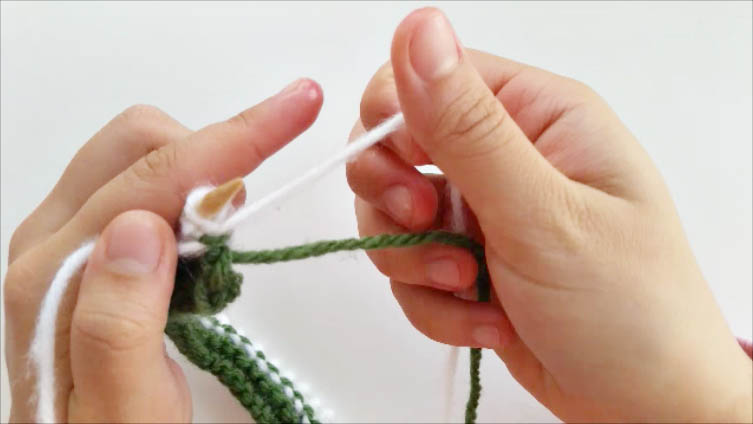
\includegraphics[width=2.5in]{step2_cross.jpg}
\end{enumerate}

\vfill \columnbreak

\subsection*{Carrying Yarn}
\begin{enumerate}
\item At the start of a RS row, you should have two yarns. In the following picture, the most recent 2 rows were worked in green (top) and the previous 2 rows were worked in white (bottom).

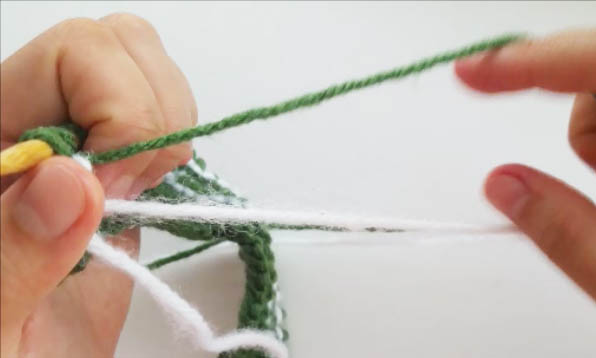
\includegraphics[width=2.5in]{step5_cross.jpg}

\item Cross the top and bottom yarns by twisting once. The direction of the twist does not matter, as long as you are consistent throughout your work. If you are switching colors for this row, skip Step 3 and work the next 2 rows in the new top color.

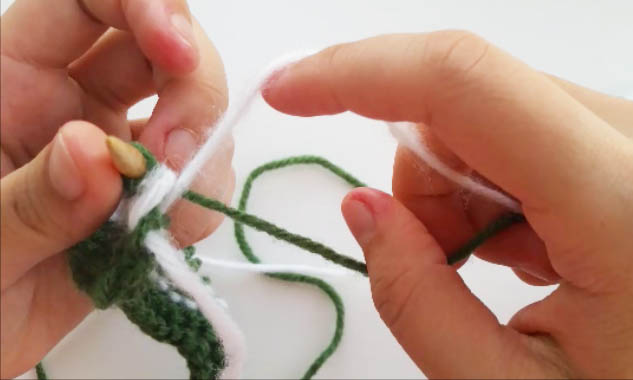
\includegraphics[width=2.5in]{step5_cross1.jpg}

\item If you are not switching colors, twist the top and bottom yarns again to cross them a second time. Work the next 2 rows in the top color (which has not changed).

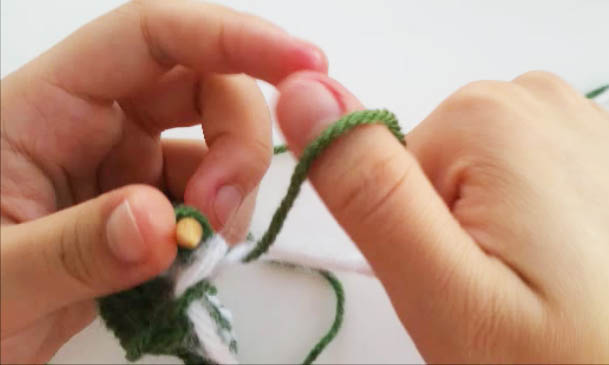
\includegraphics[width=2.5in]{step6_cross2.jpg}

\end{enumerate}
\end{multicols}

\newpage
\section*{Appendix B: Right and Left Twists (Mini-Cables)}

The method in this tutorial shows you how to create a true 1x1 cable without a cable needle. The right and left twists are worked over two stitches, labeled as Stitch 1 (S1, \emph{blue}) and Stitch 2 (S2, \emph{red}) in the photos. Working yarn is labeled in \emph{green}.

\subsection*{Left Twist}

\begin{multicols}{2}
\begin{enumerate}
\item Insert needle between S1 and S2 from behind.

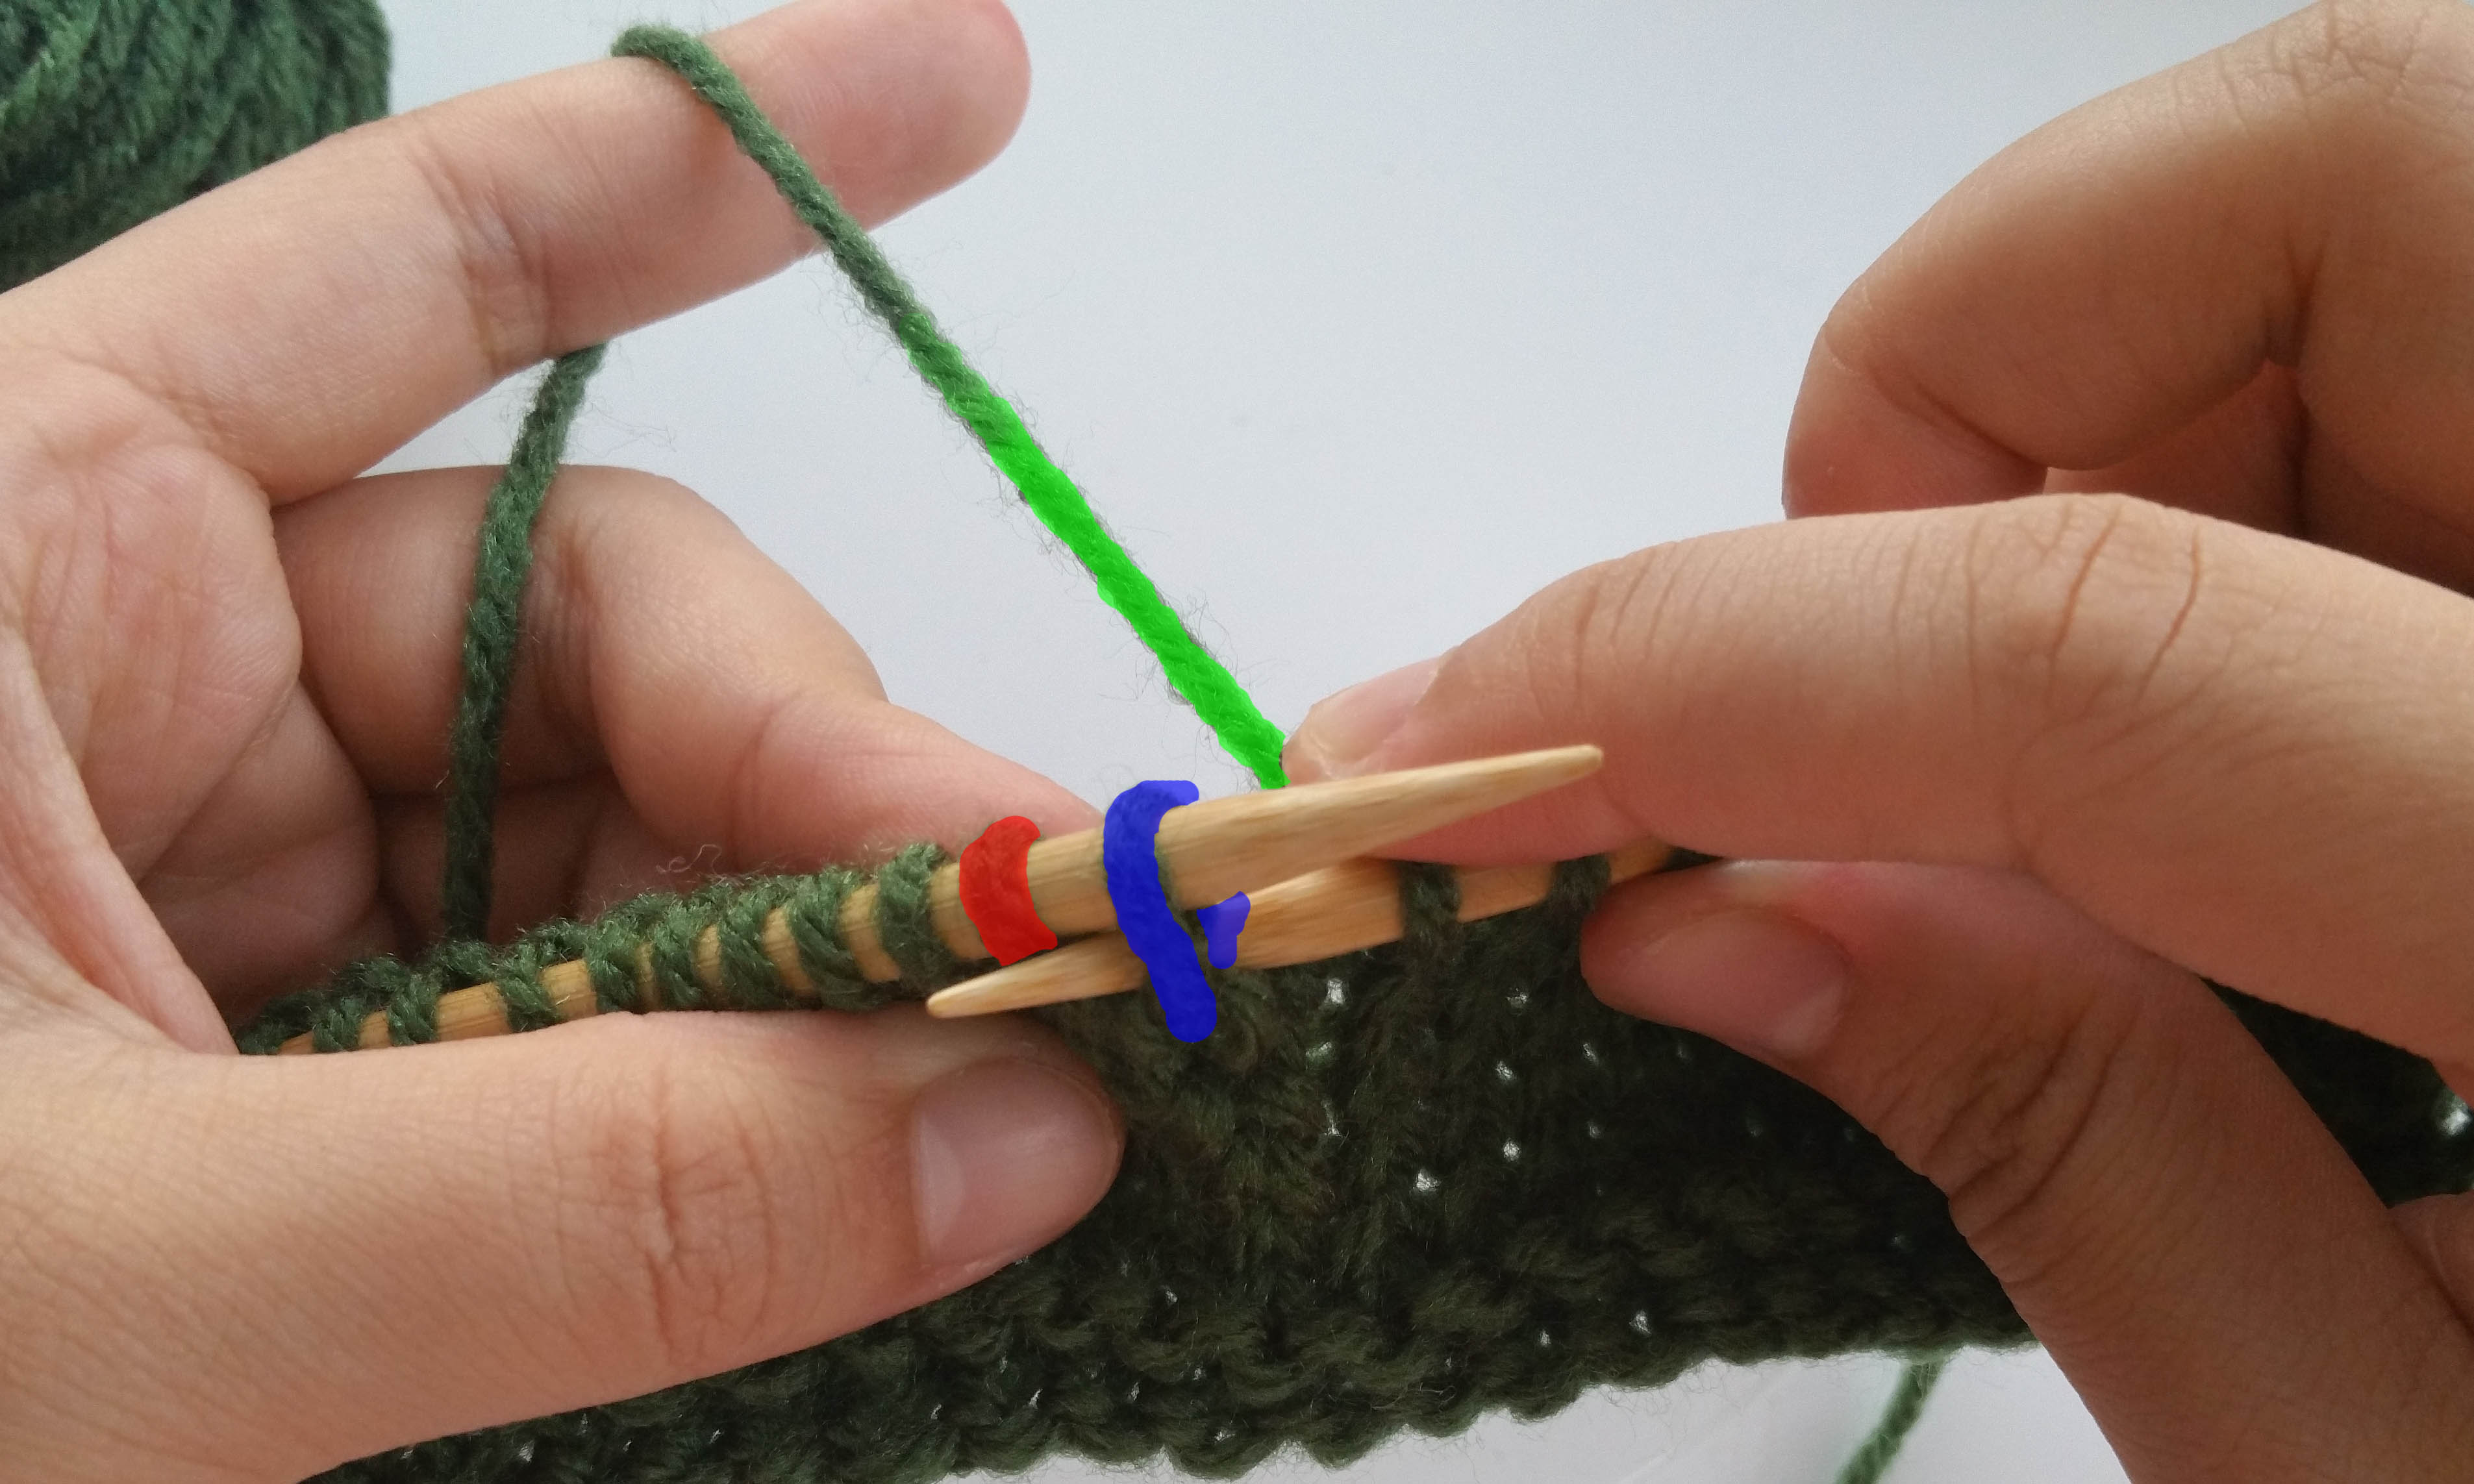
\includegraphics[width=2.5in]{lt_step1.jpg}

\item Knit into S2, keeping both stitches on the left needle. The new stitch will be in front of the work.

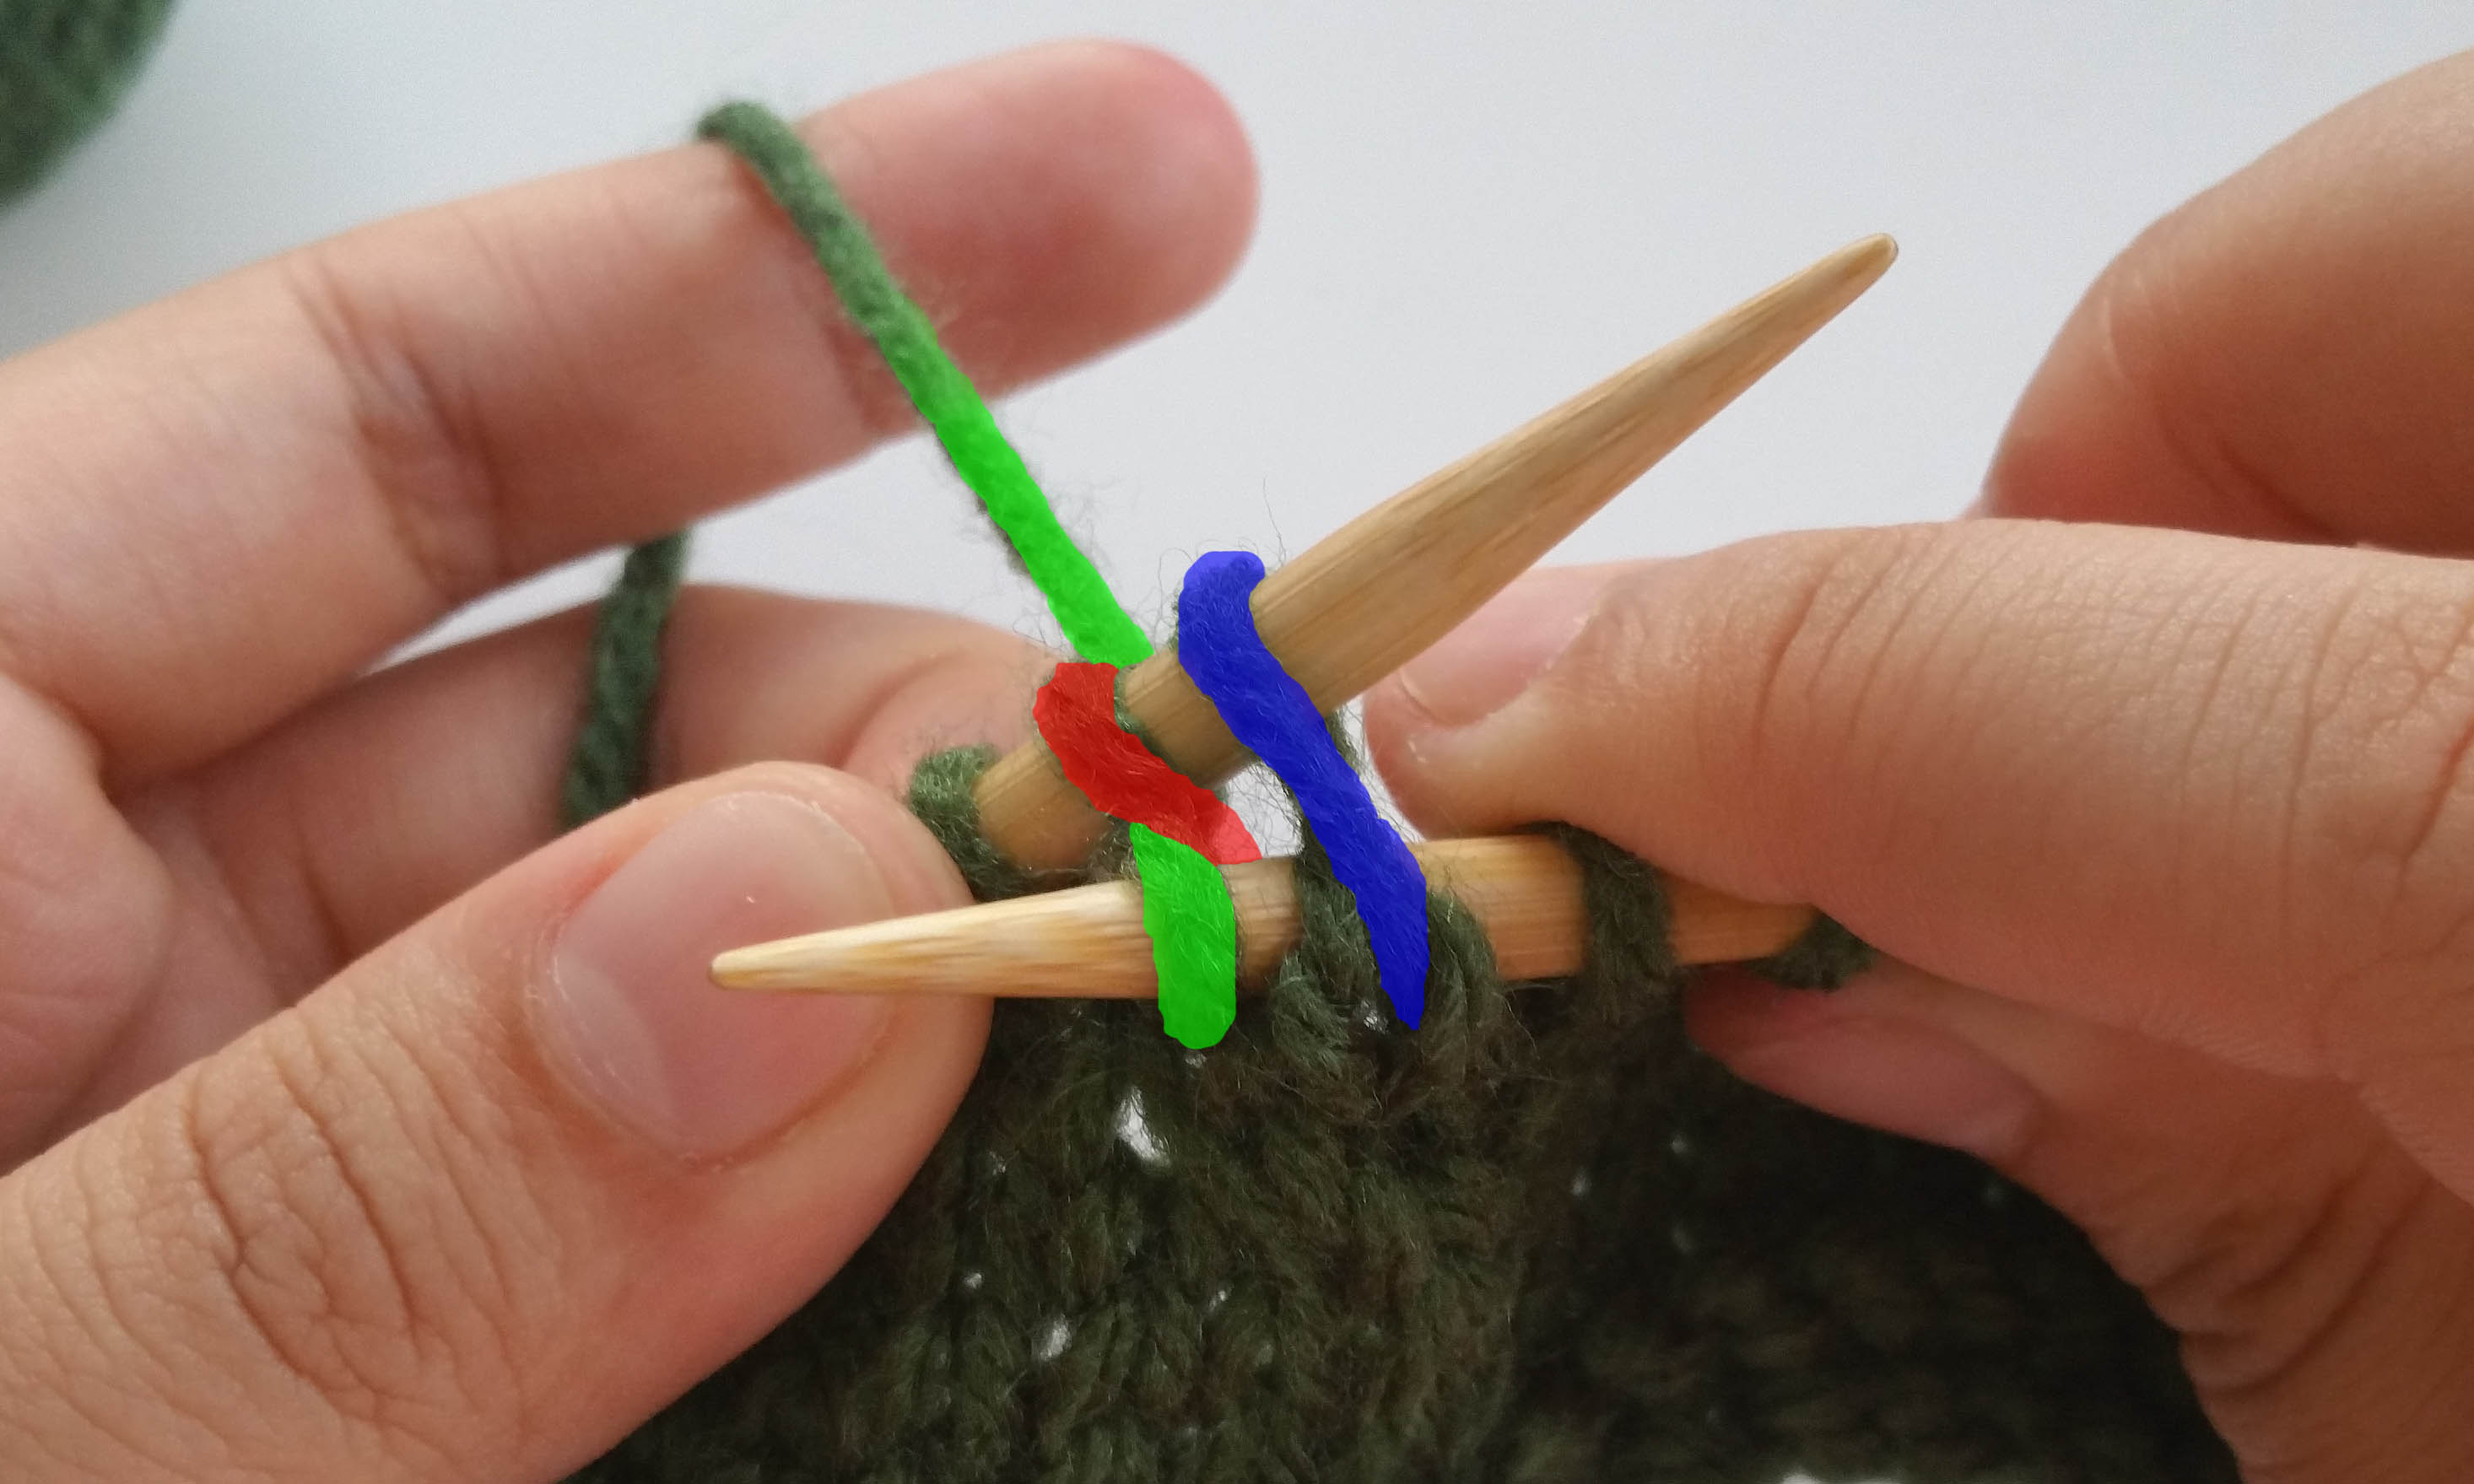
\includegraphics[width=2.5in]{lt_step2.jpg}

\item Bring right needle behind work by going back between S1 and S2.

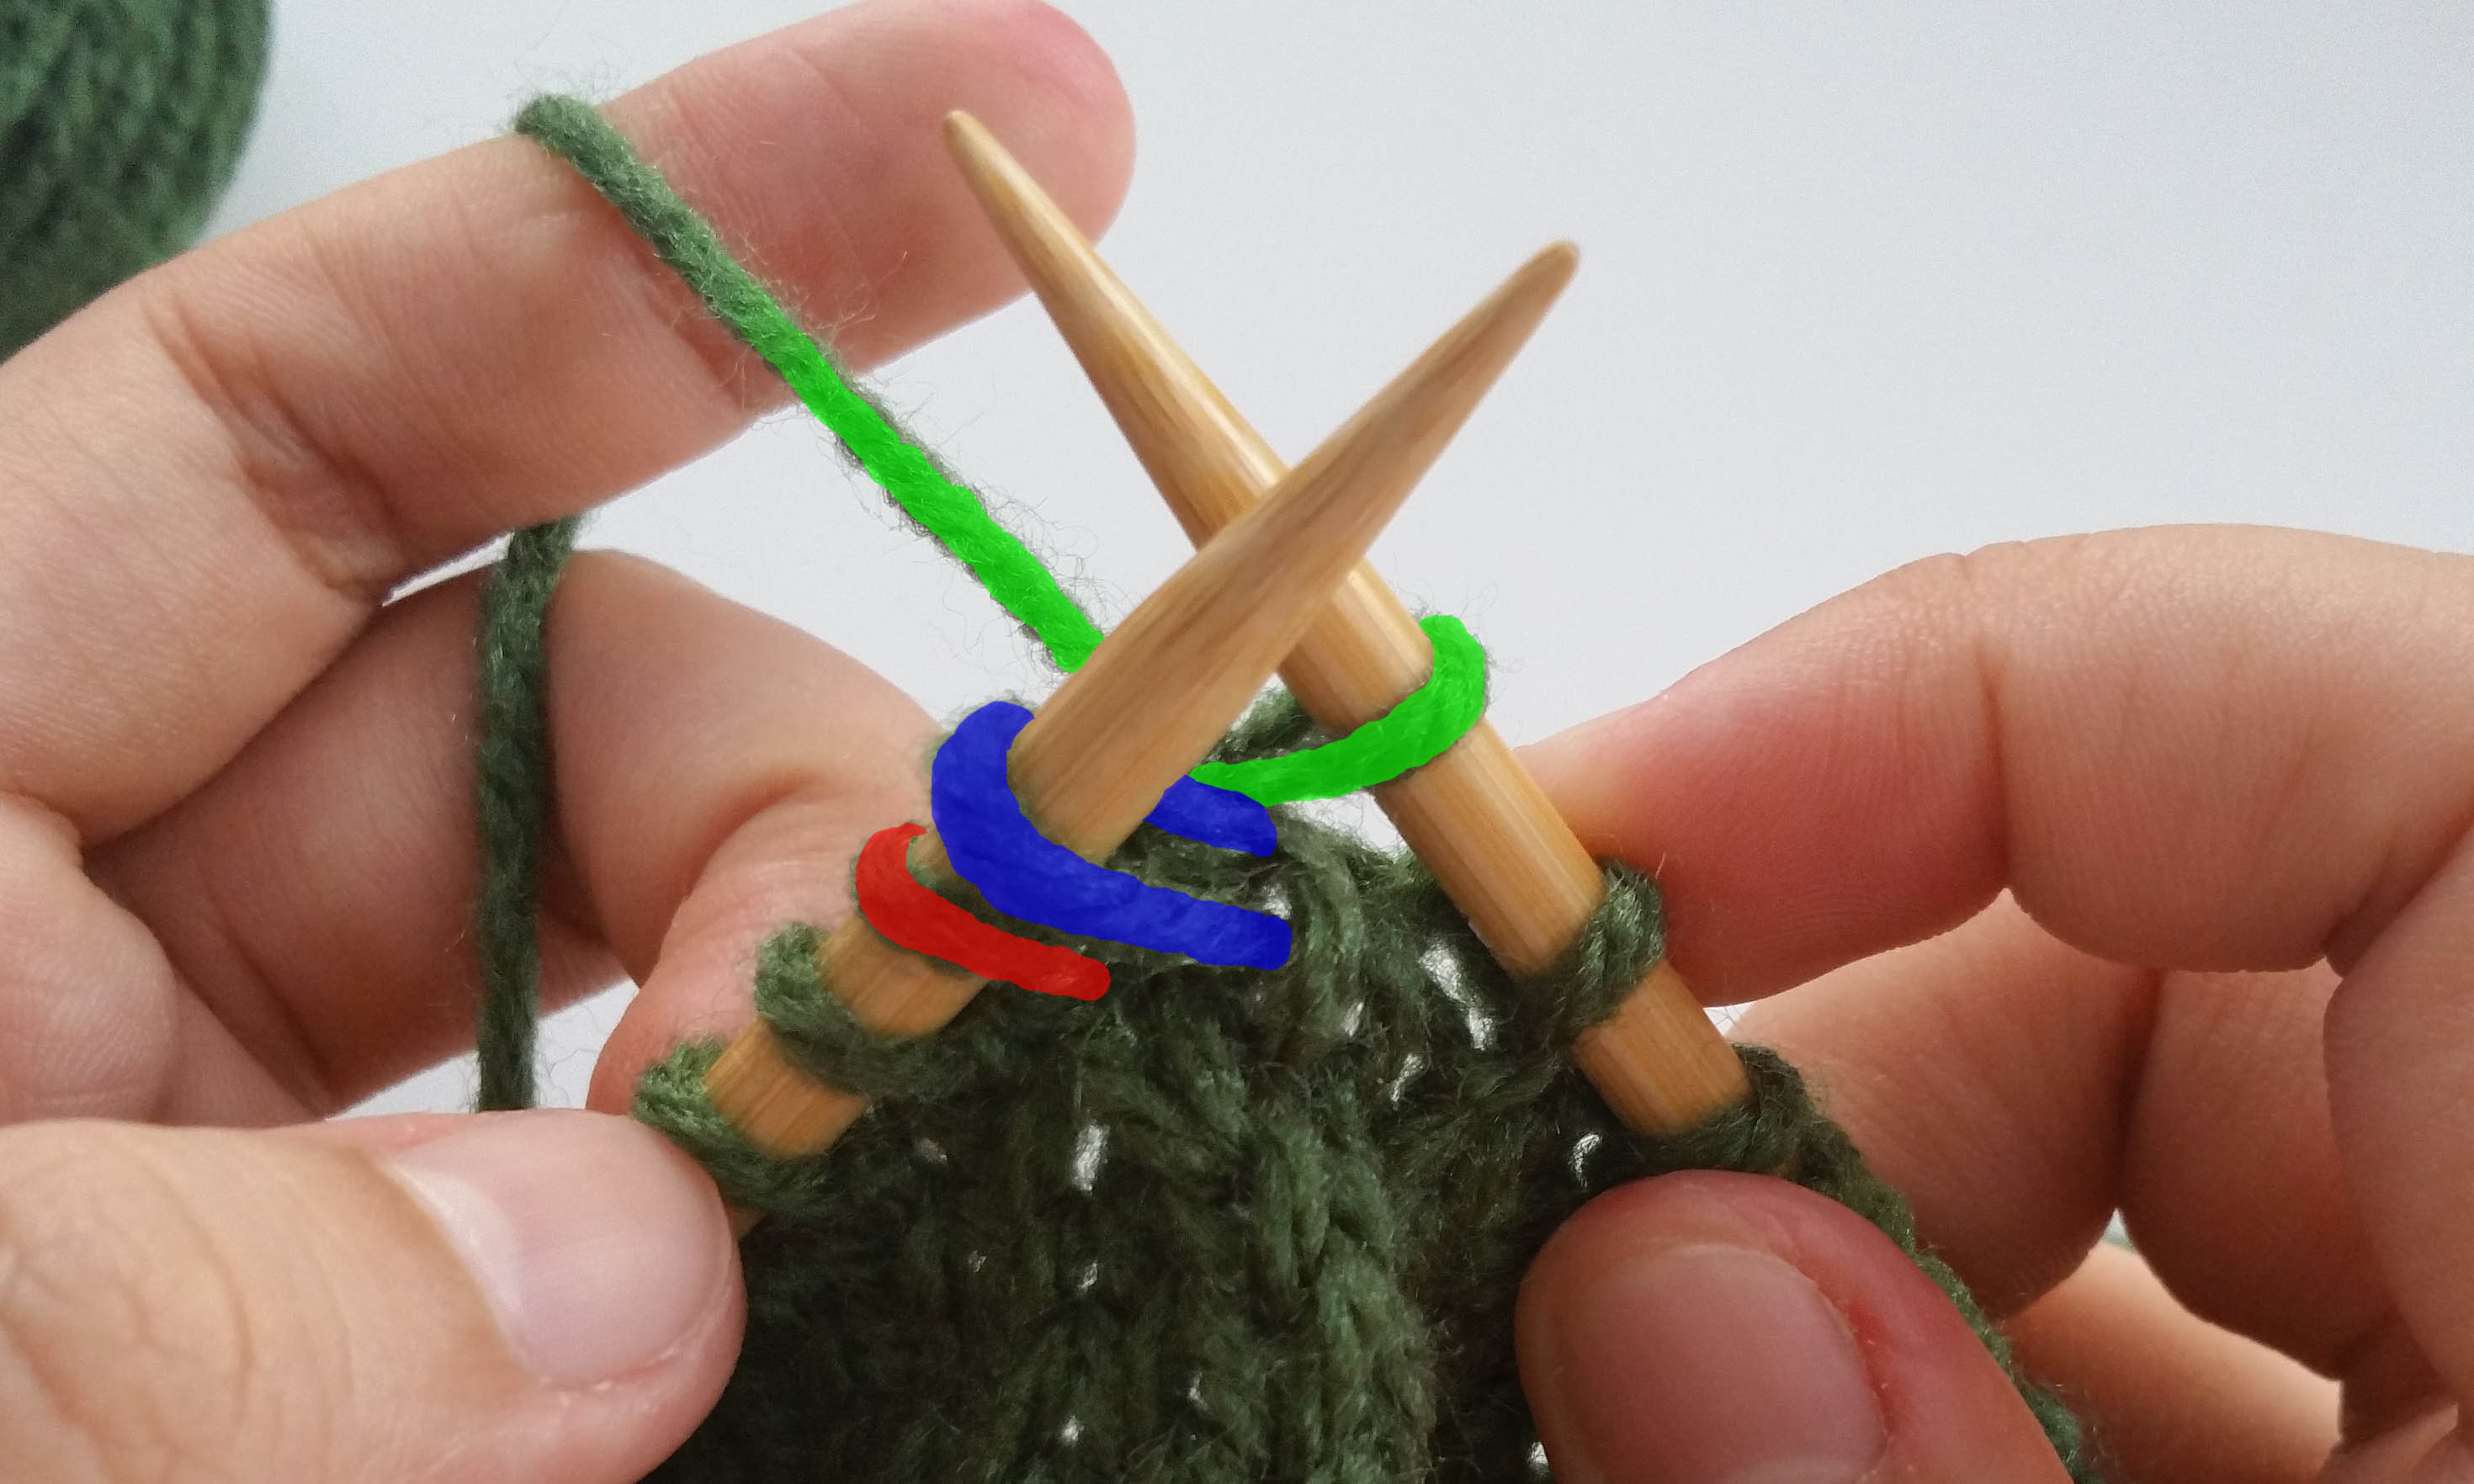
\includegraphics[width=2.5in]{lt_step3.jpg}

\vfill \columnbreak

\item Bring right needle to front of work and knit into S1.

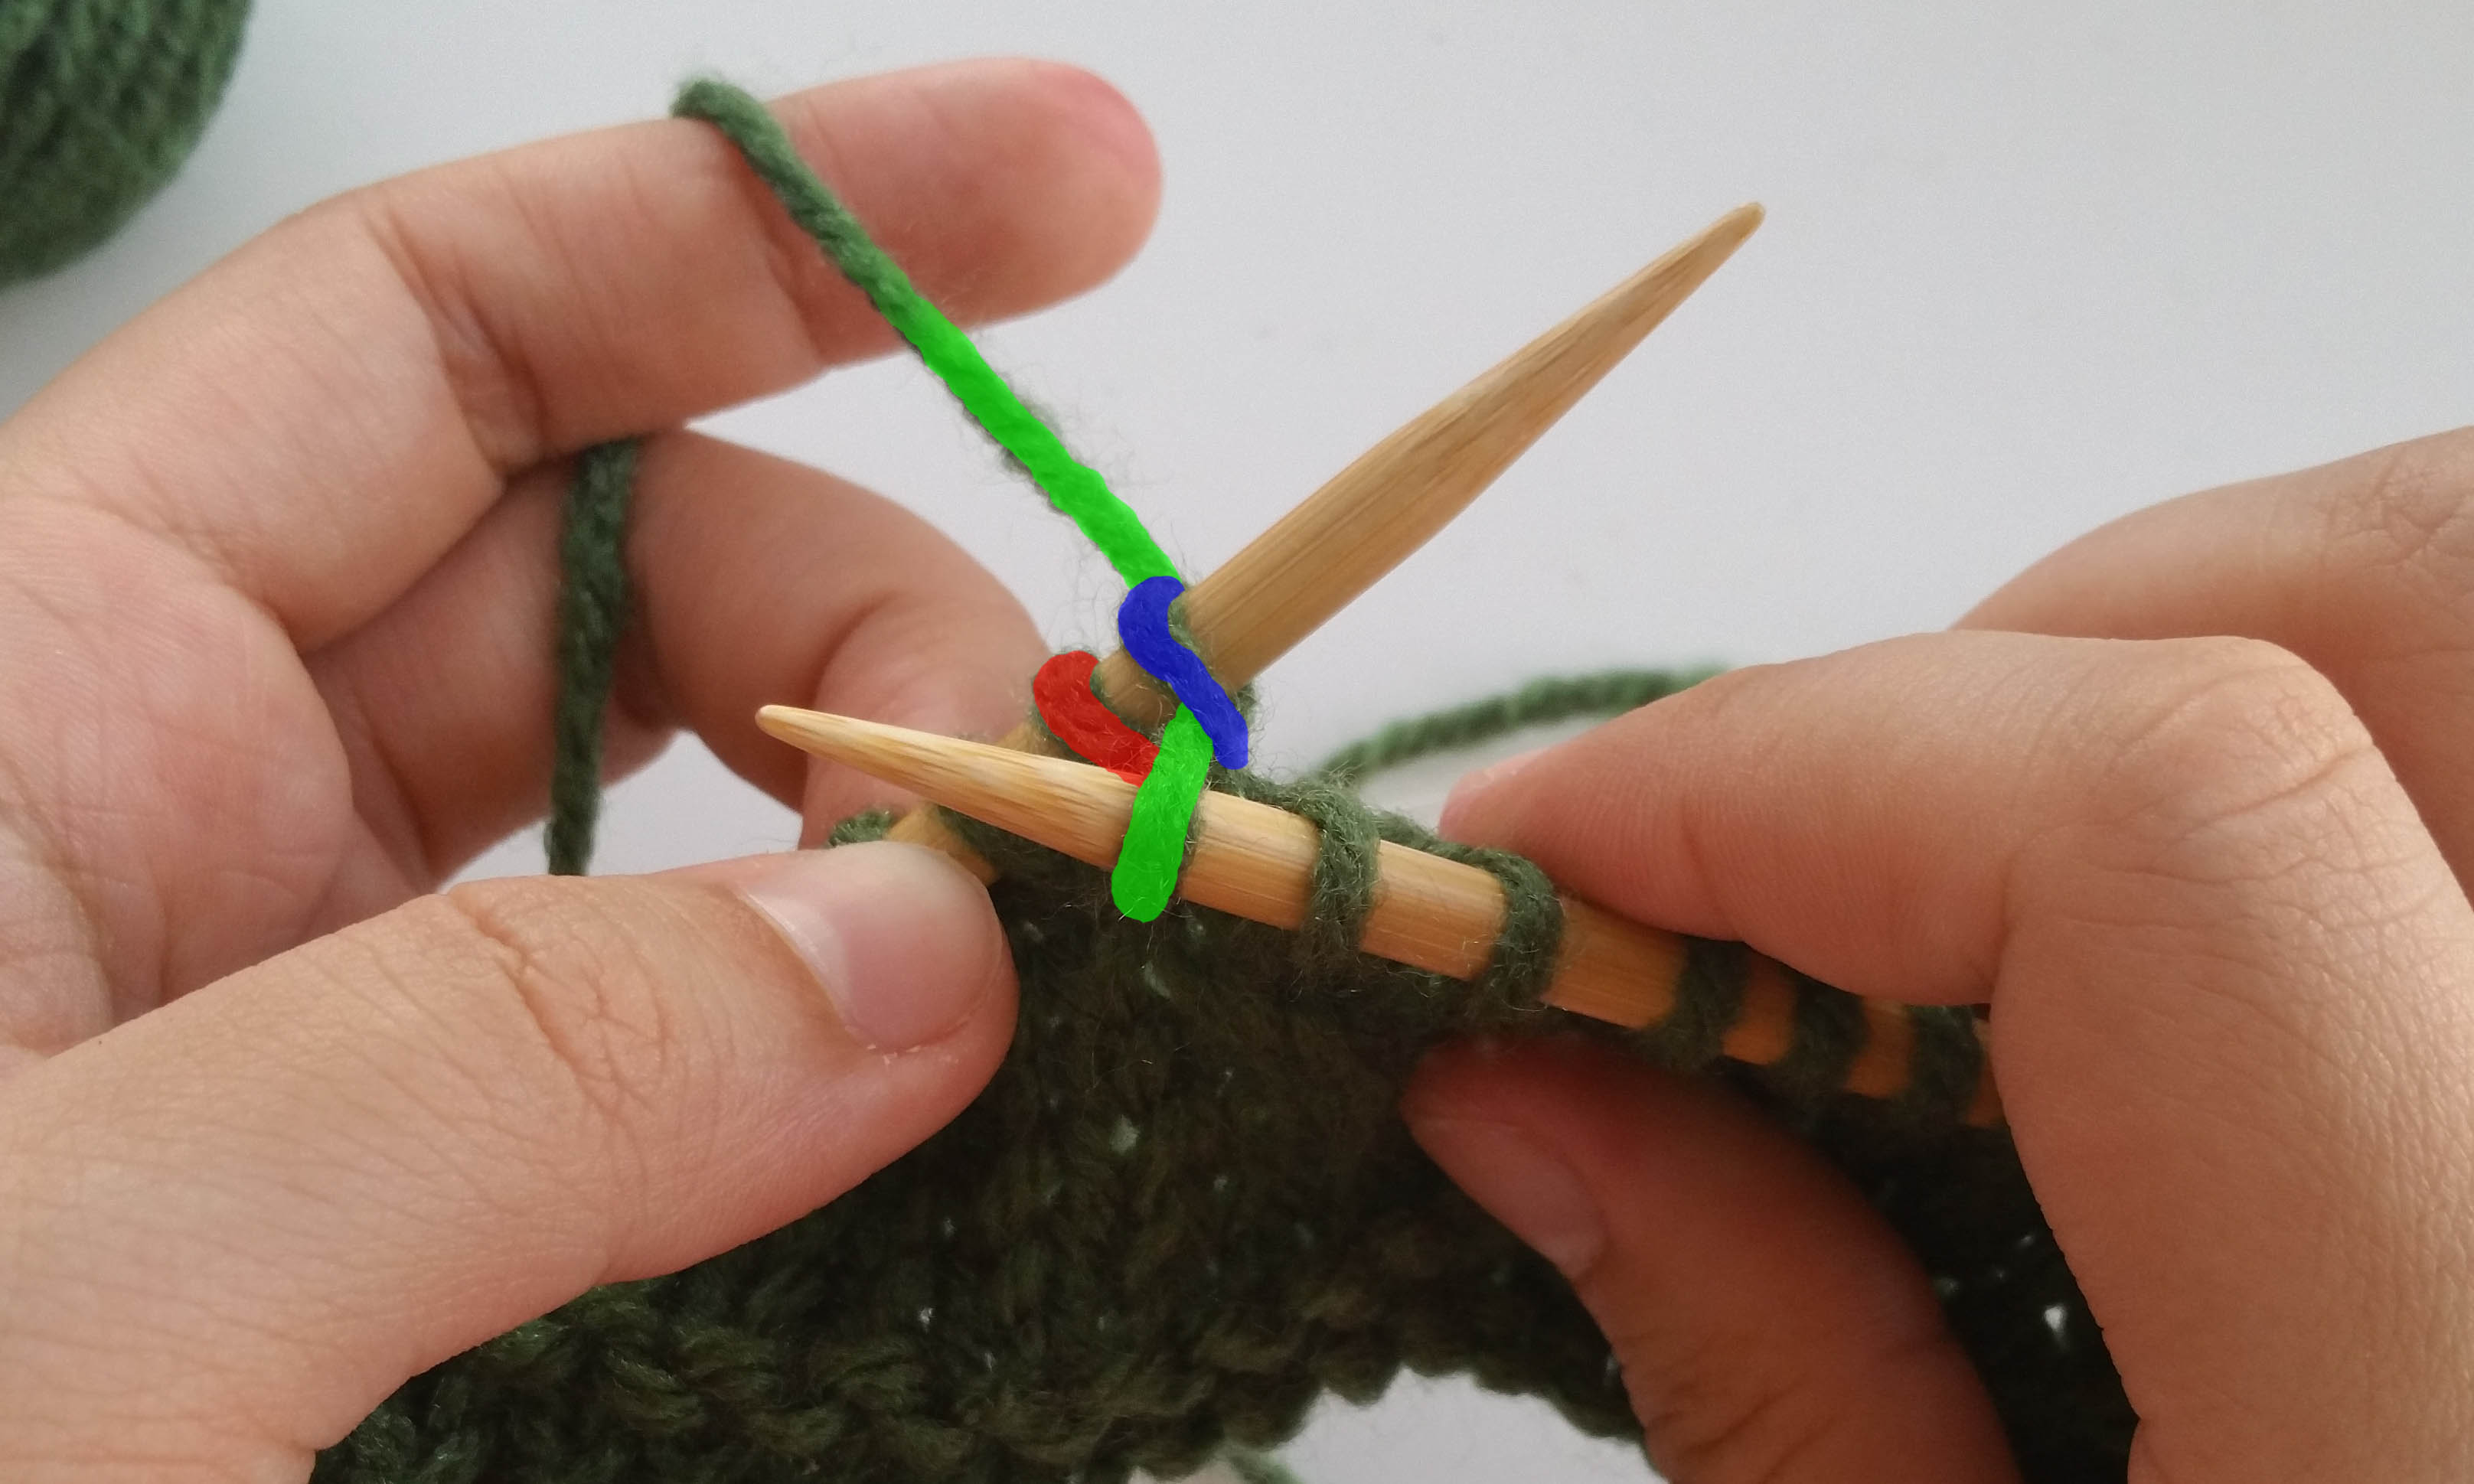
\includegraphics[width=2.5in]{lt_step4.jpg}

\item Drop both stitches off the left needle.

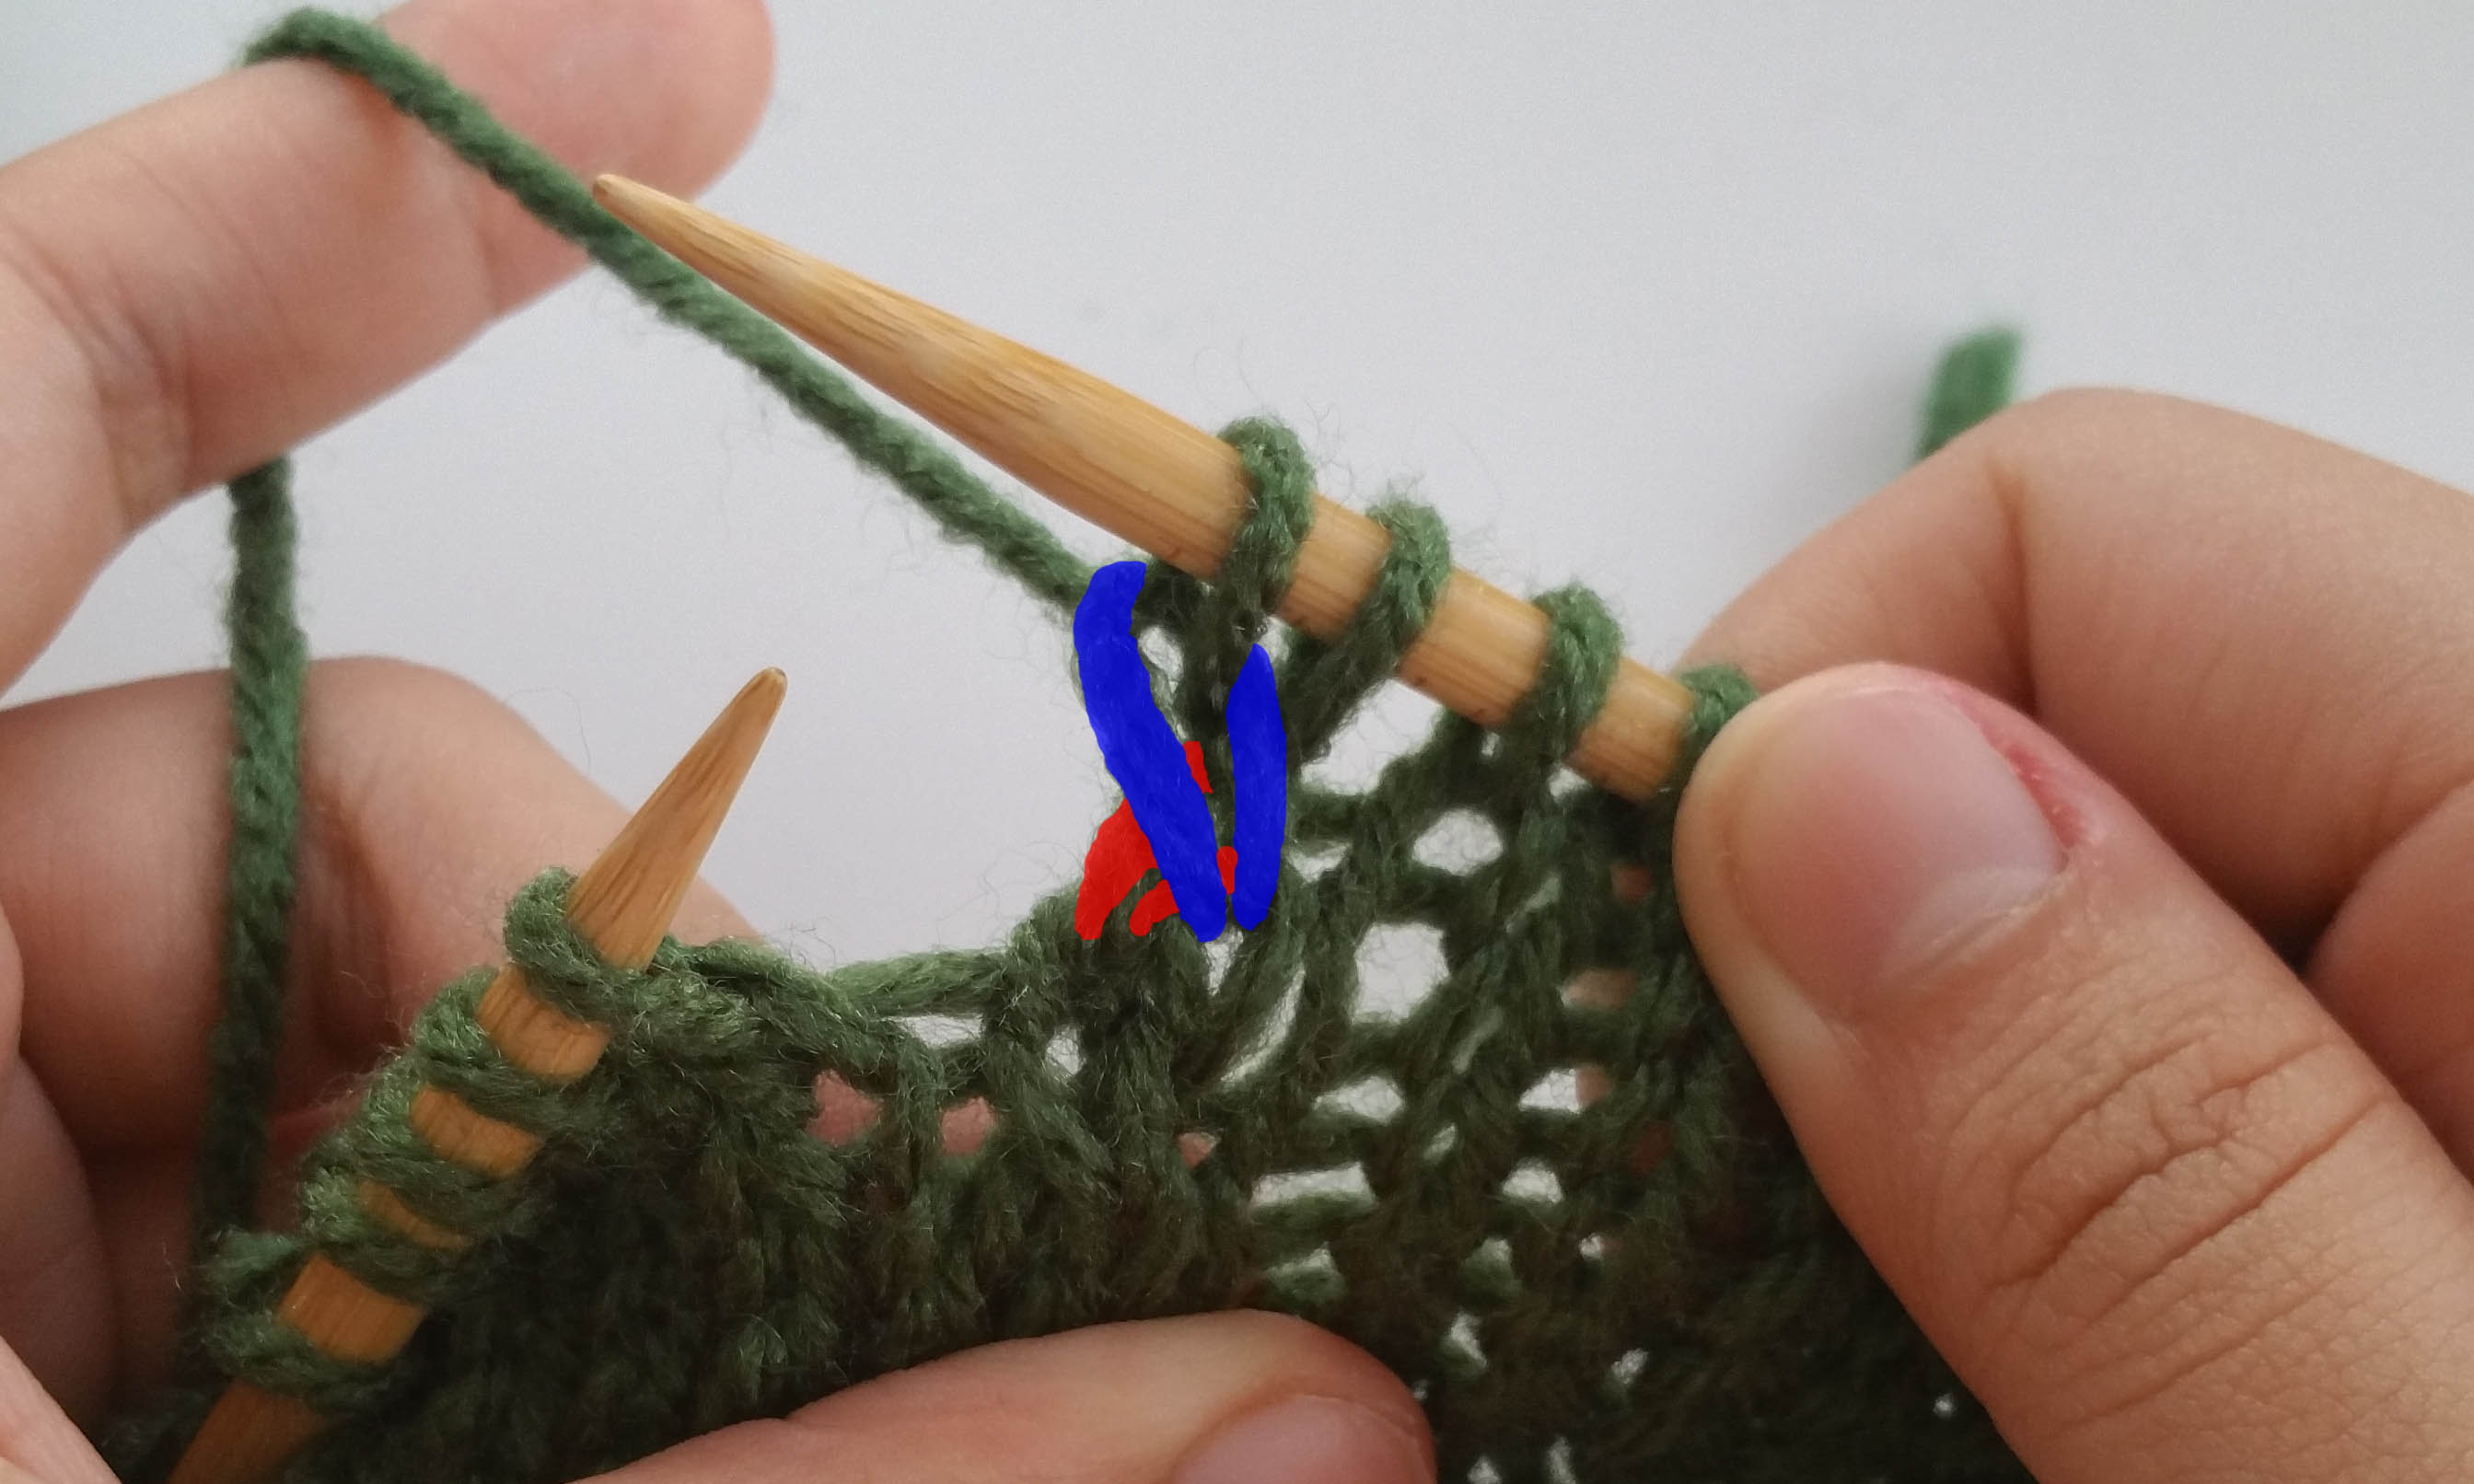
\includegraphics[width=2.5in]{lt_step5.jpg}
\end{enumerate}
\end{multicols}

\newpage

\subsection*{Right Twist}

\begin{multicols}{2}
\begin{enumerate}
\item Bring yarn to front and bring right needle in front of yarn.

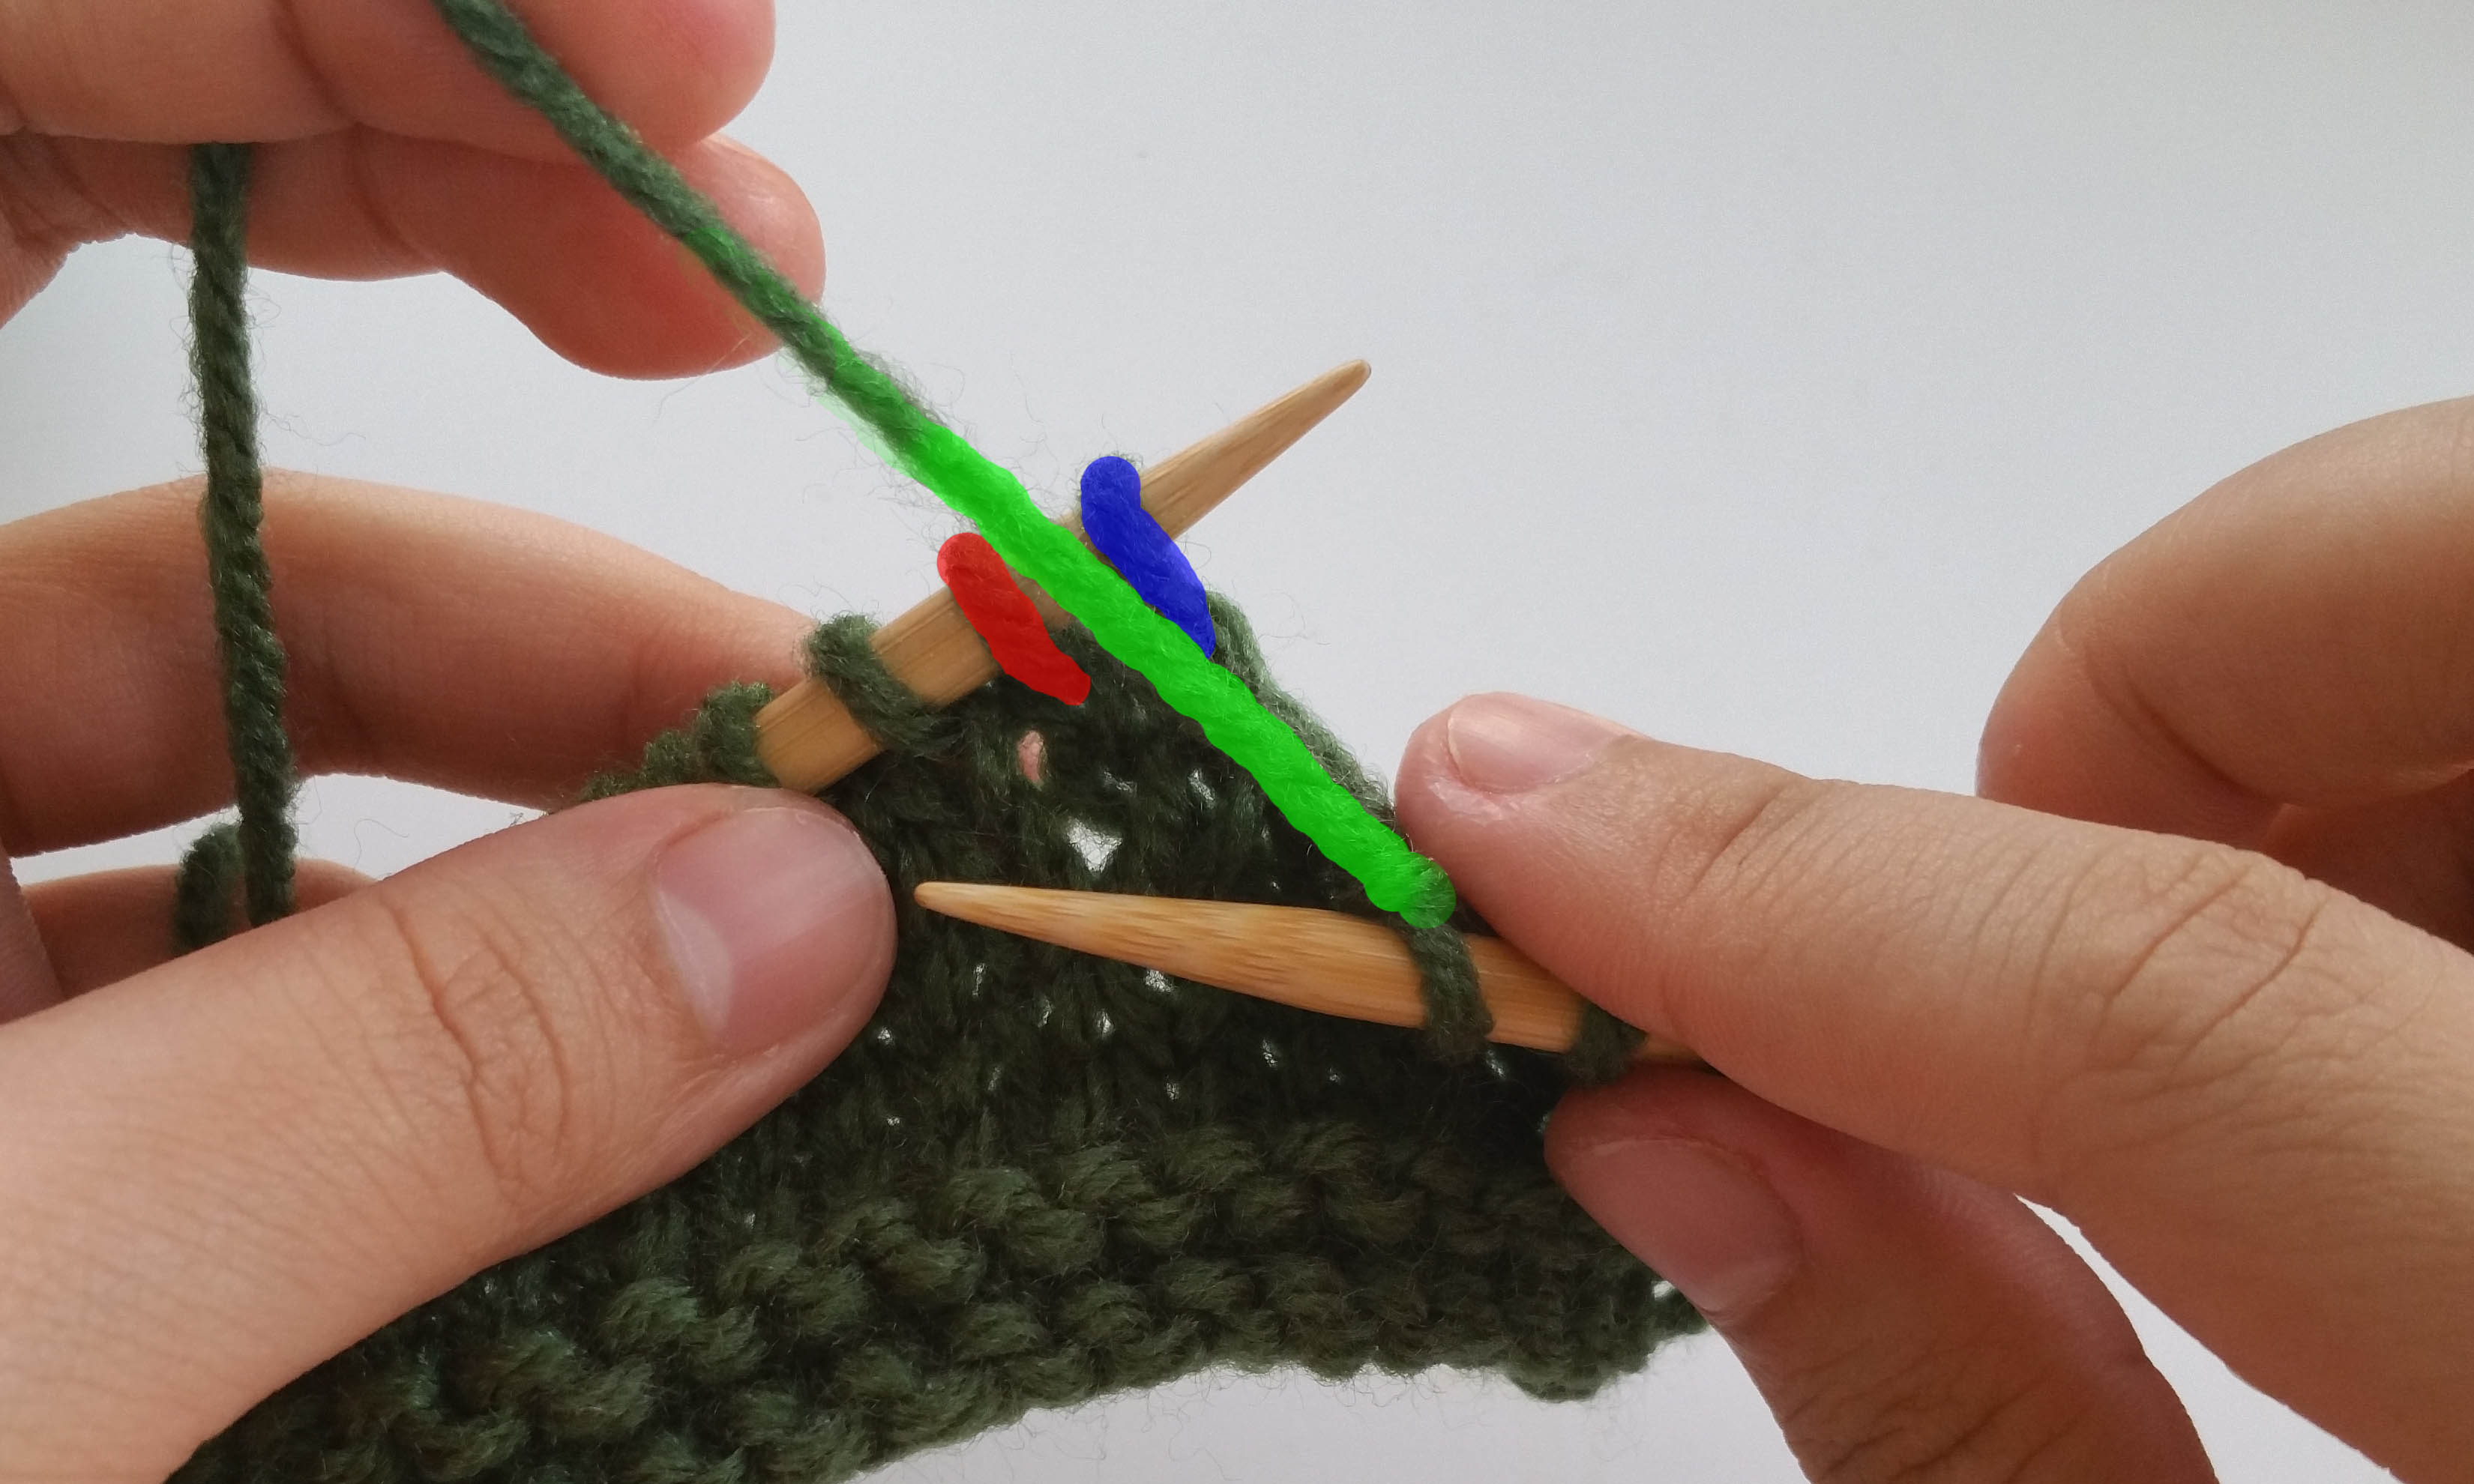
\includegraphics[width=2.5in]{rt_step1.jpg}

\item Knit into S2, keeping both yarn and needle in front.

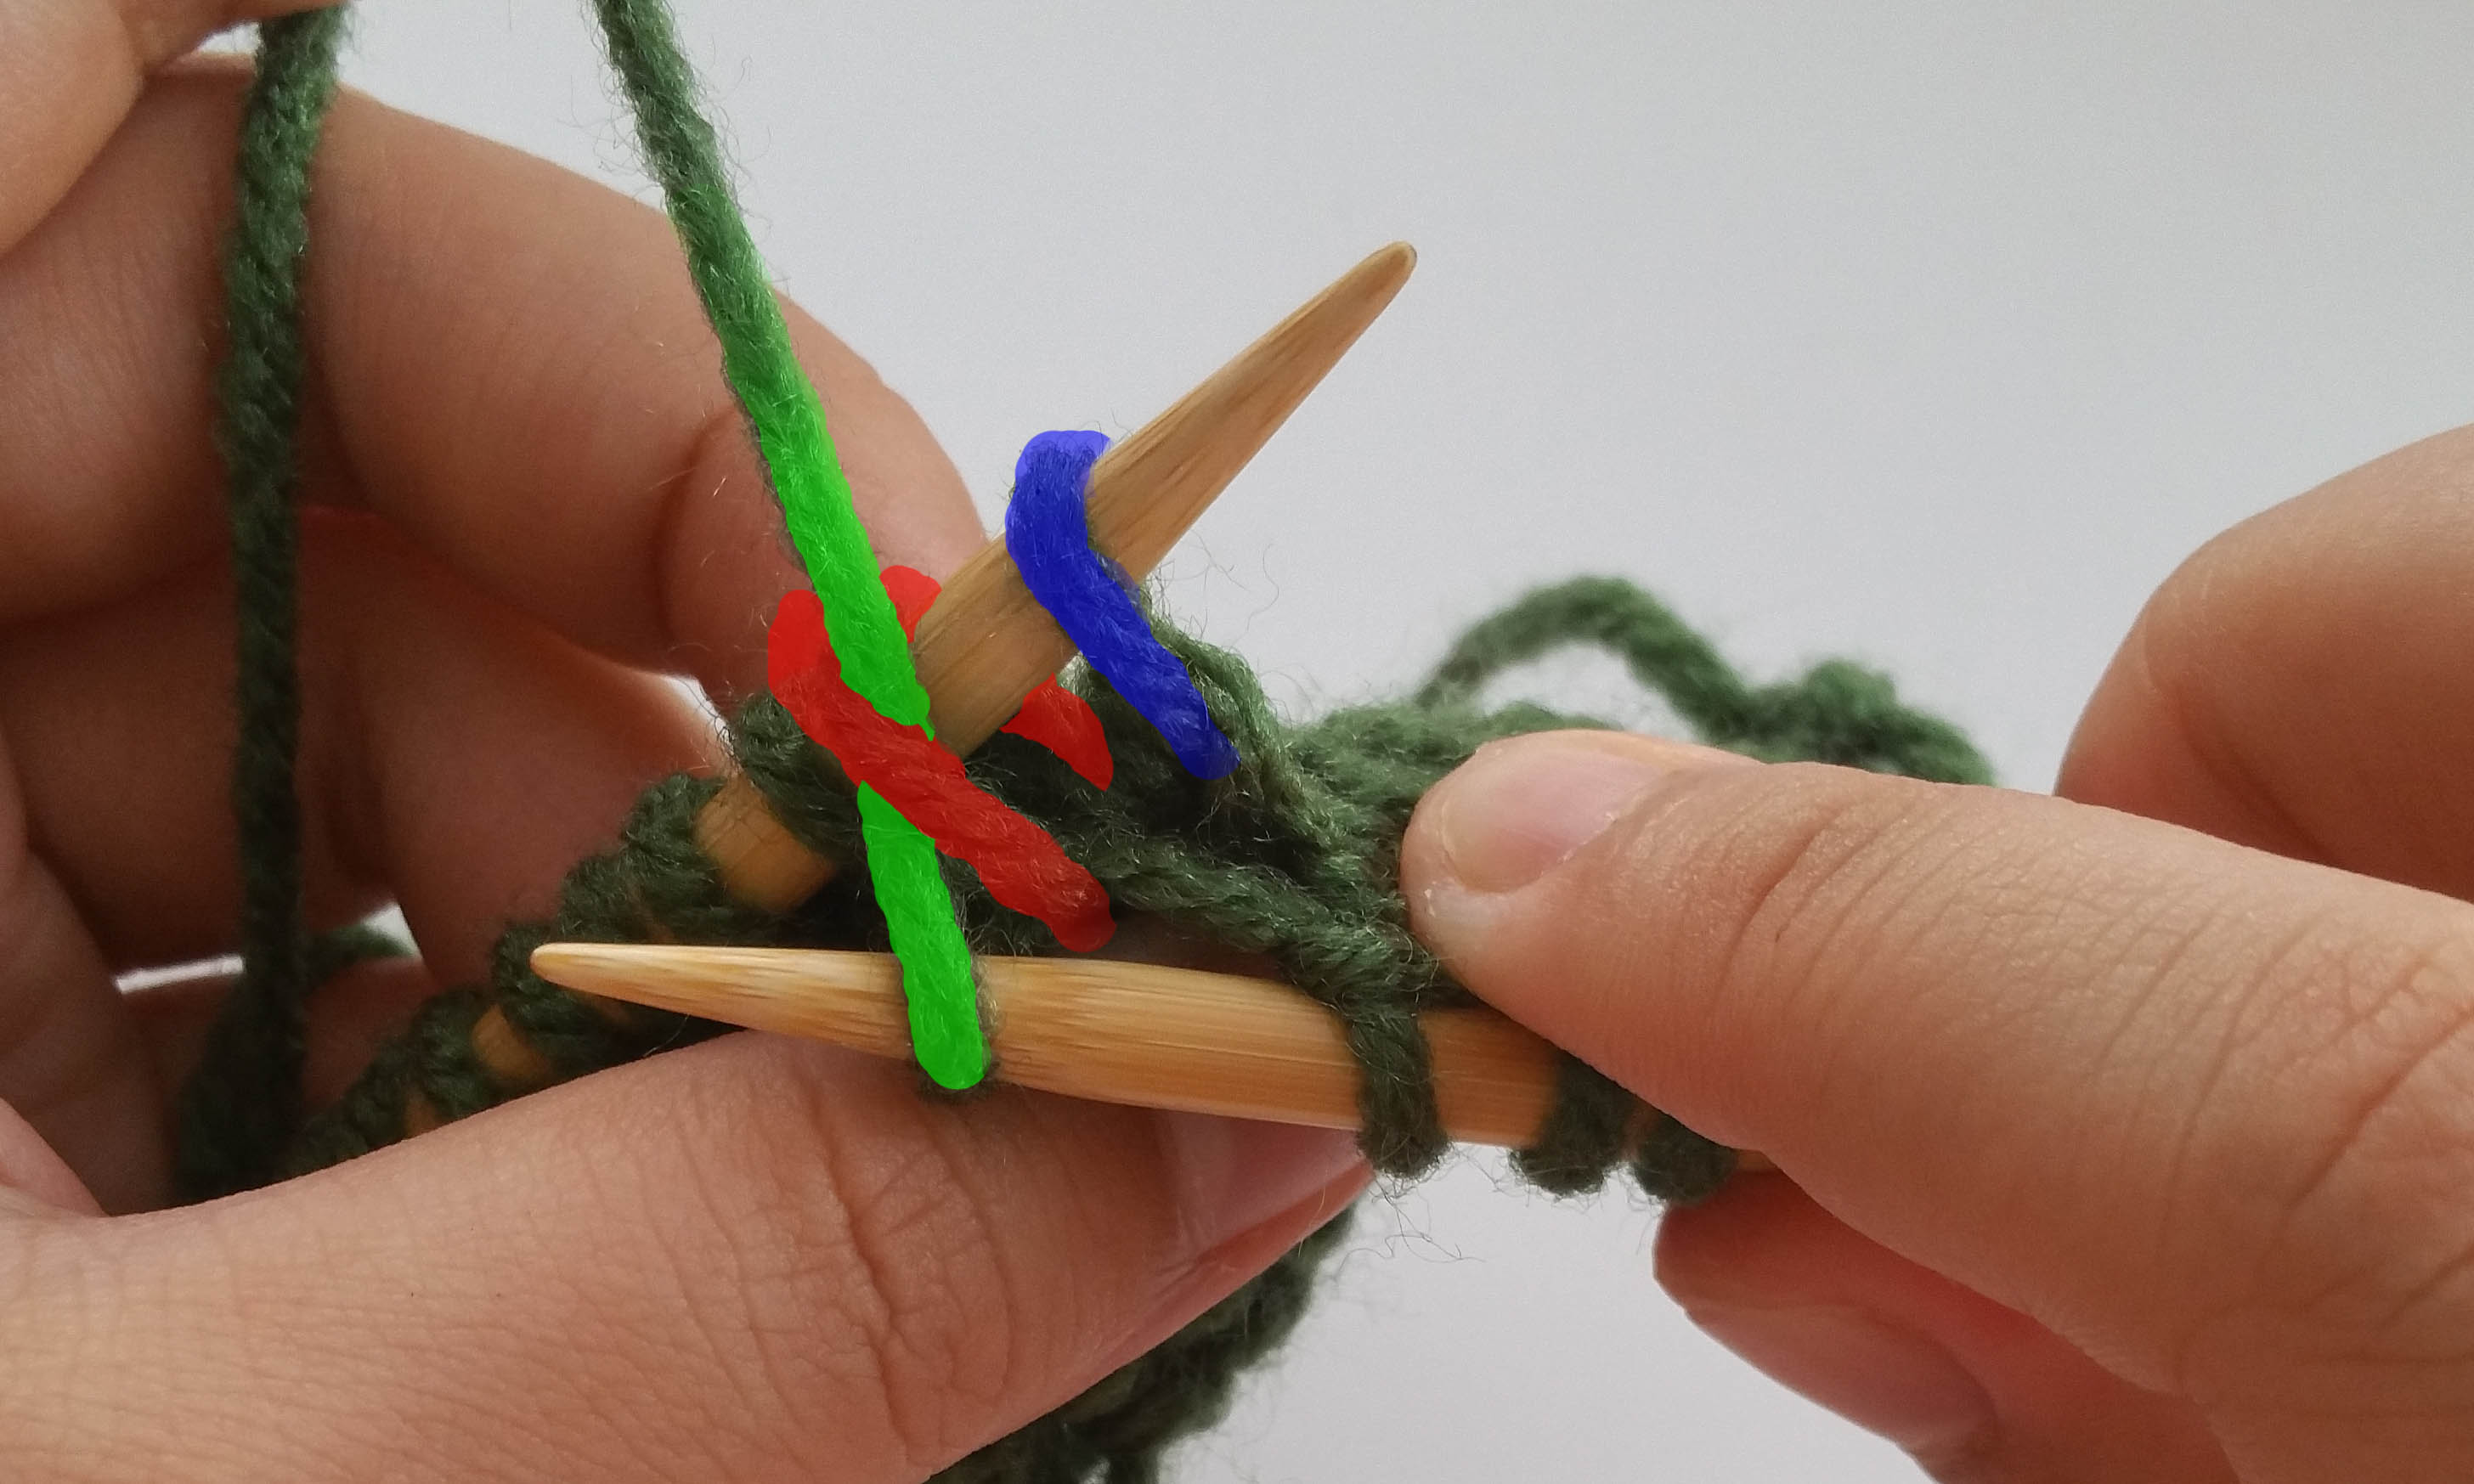
\includegraphics[width=2.5in]{rt_step2.jpg}

\item Keeping both S1 and S2 on the needle, bring working yarn to back.

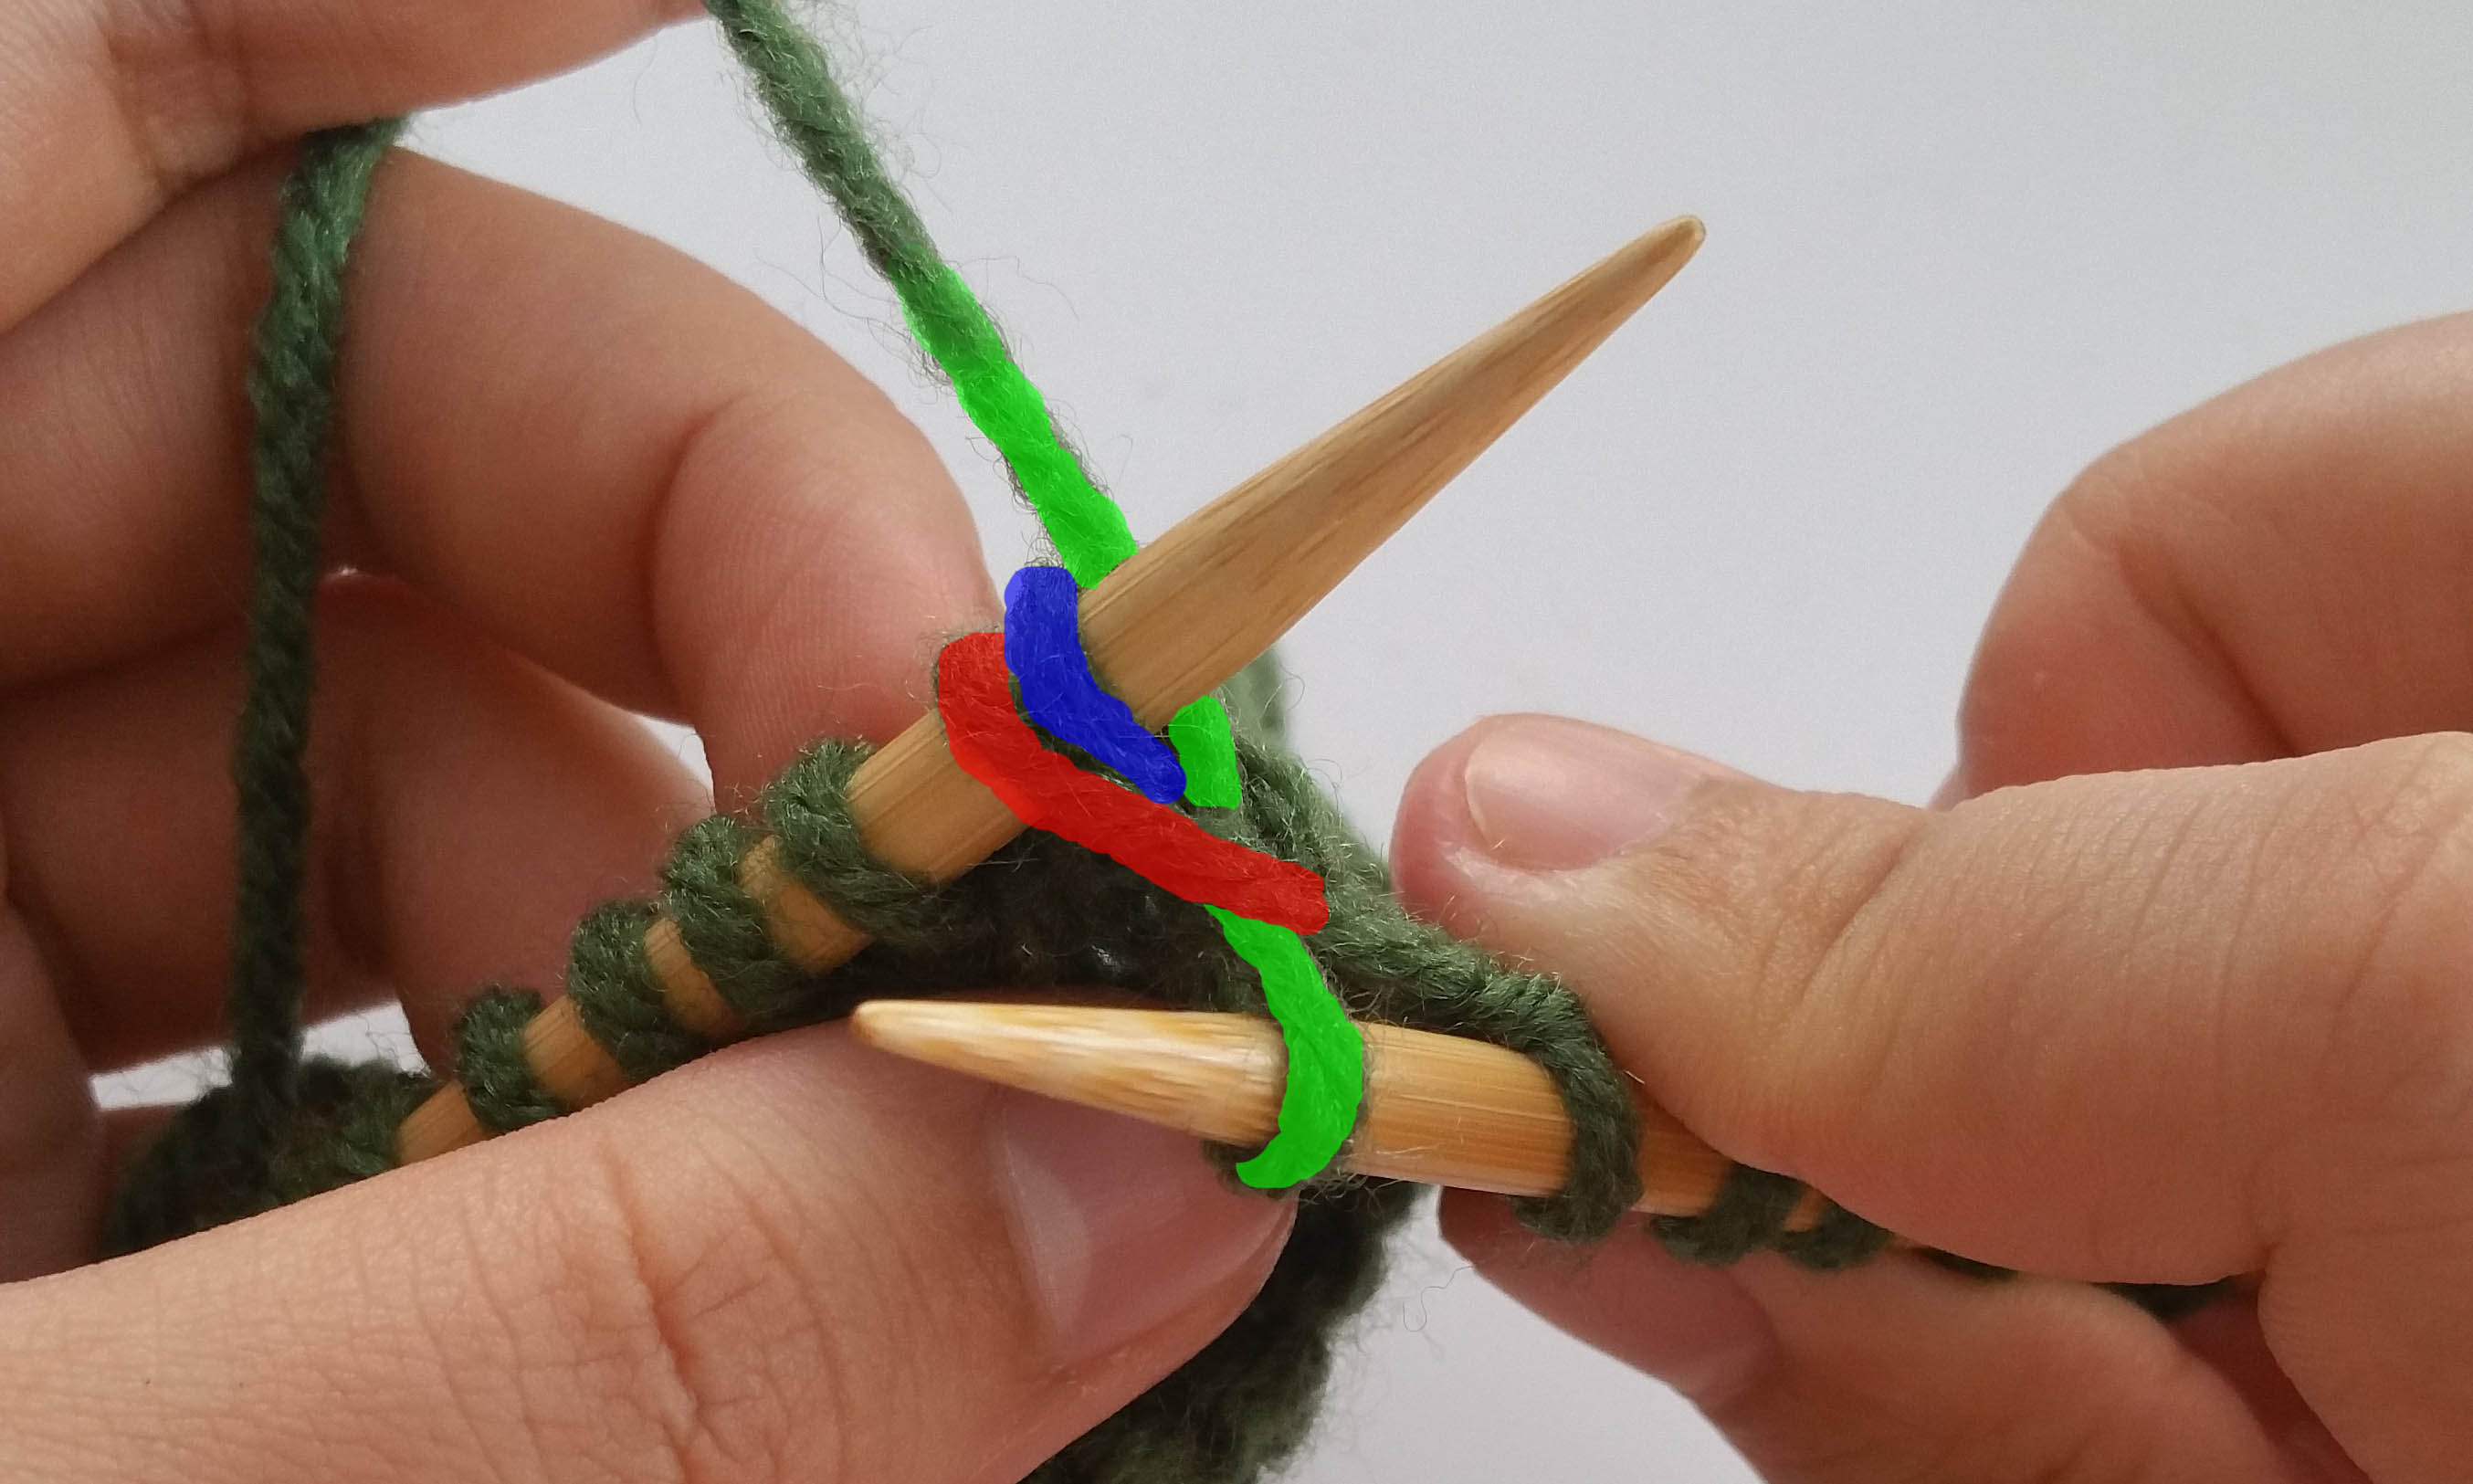
\includegraphics[width=2.5in]{rt_step3.jpg}

\vfill \columnbreak

\item Knit into S1.

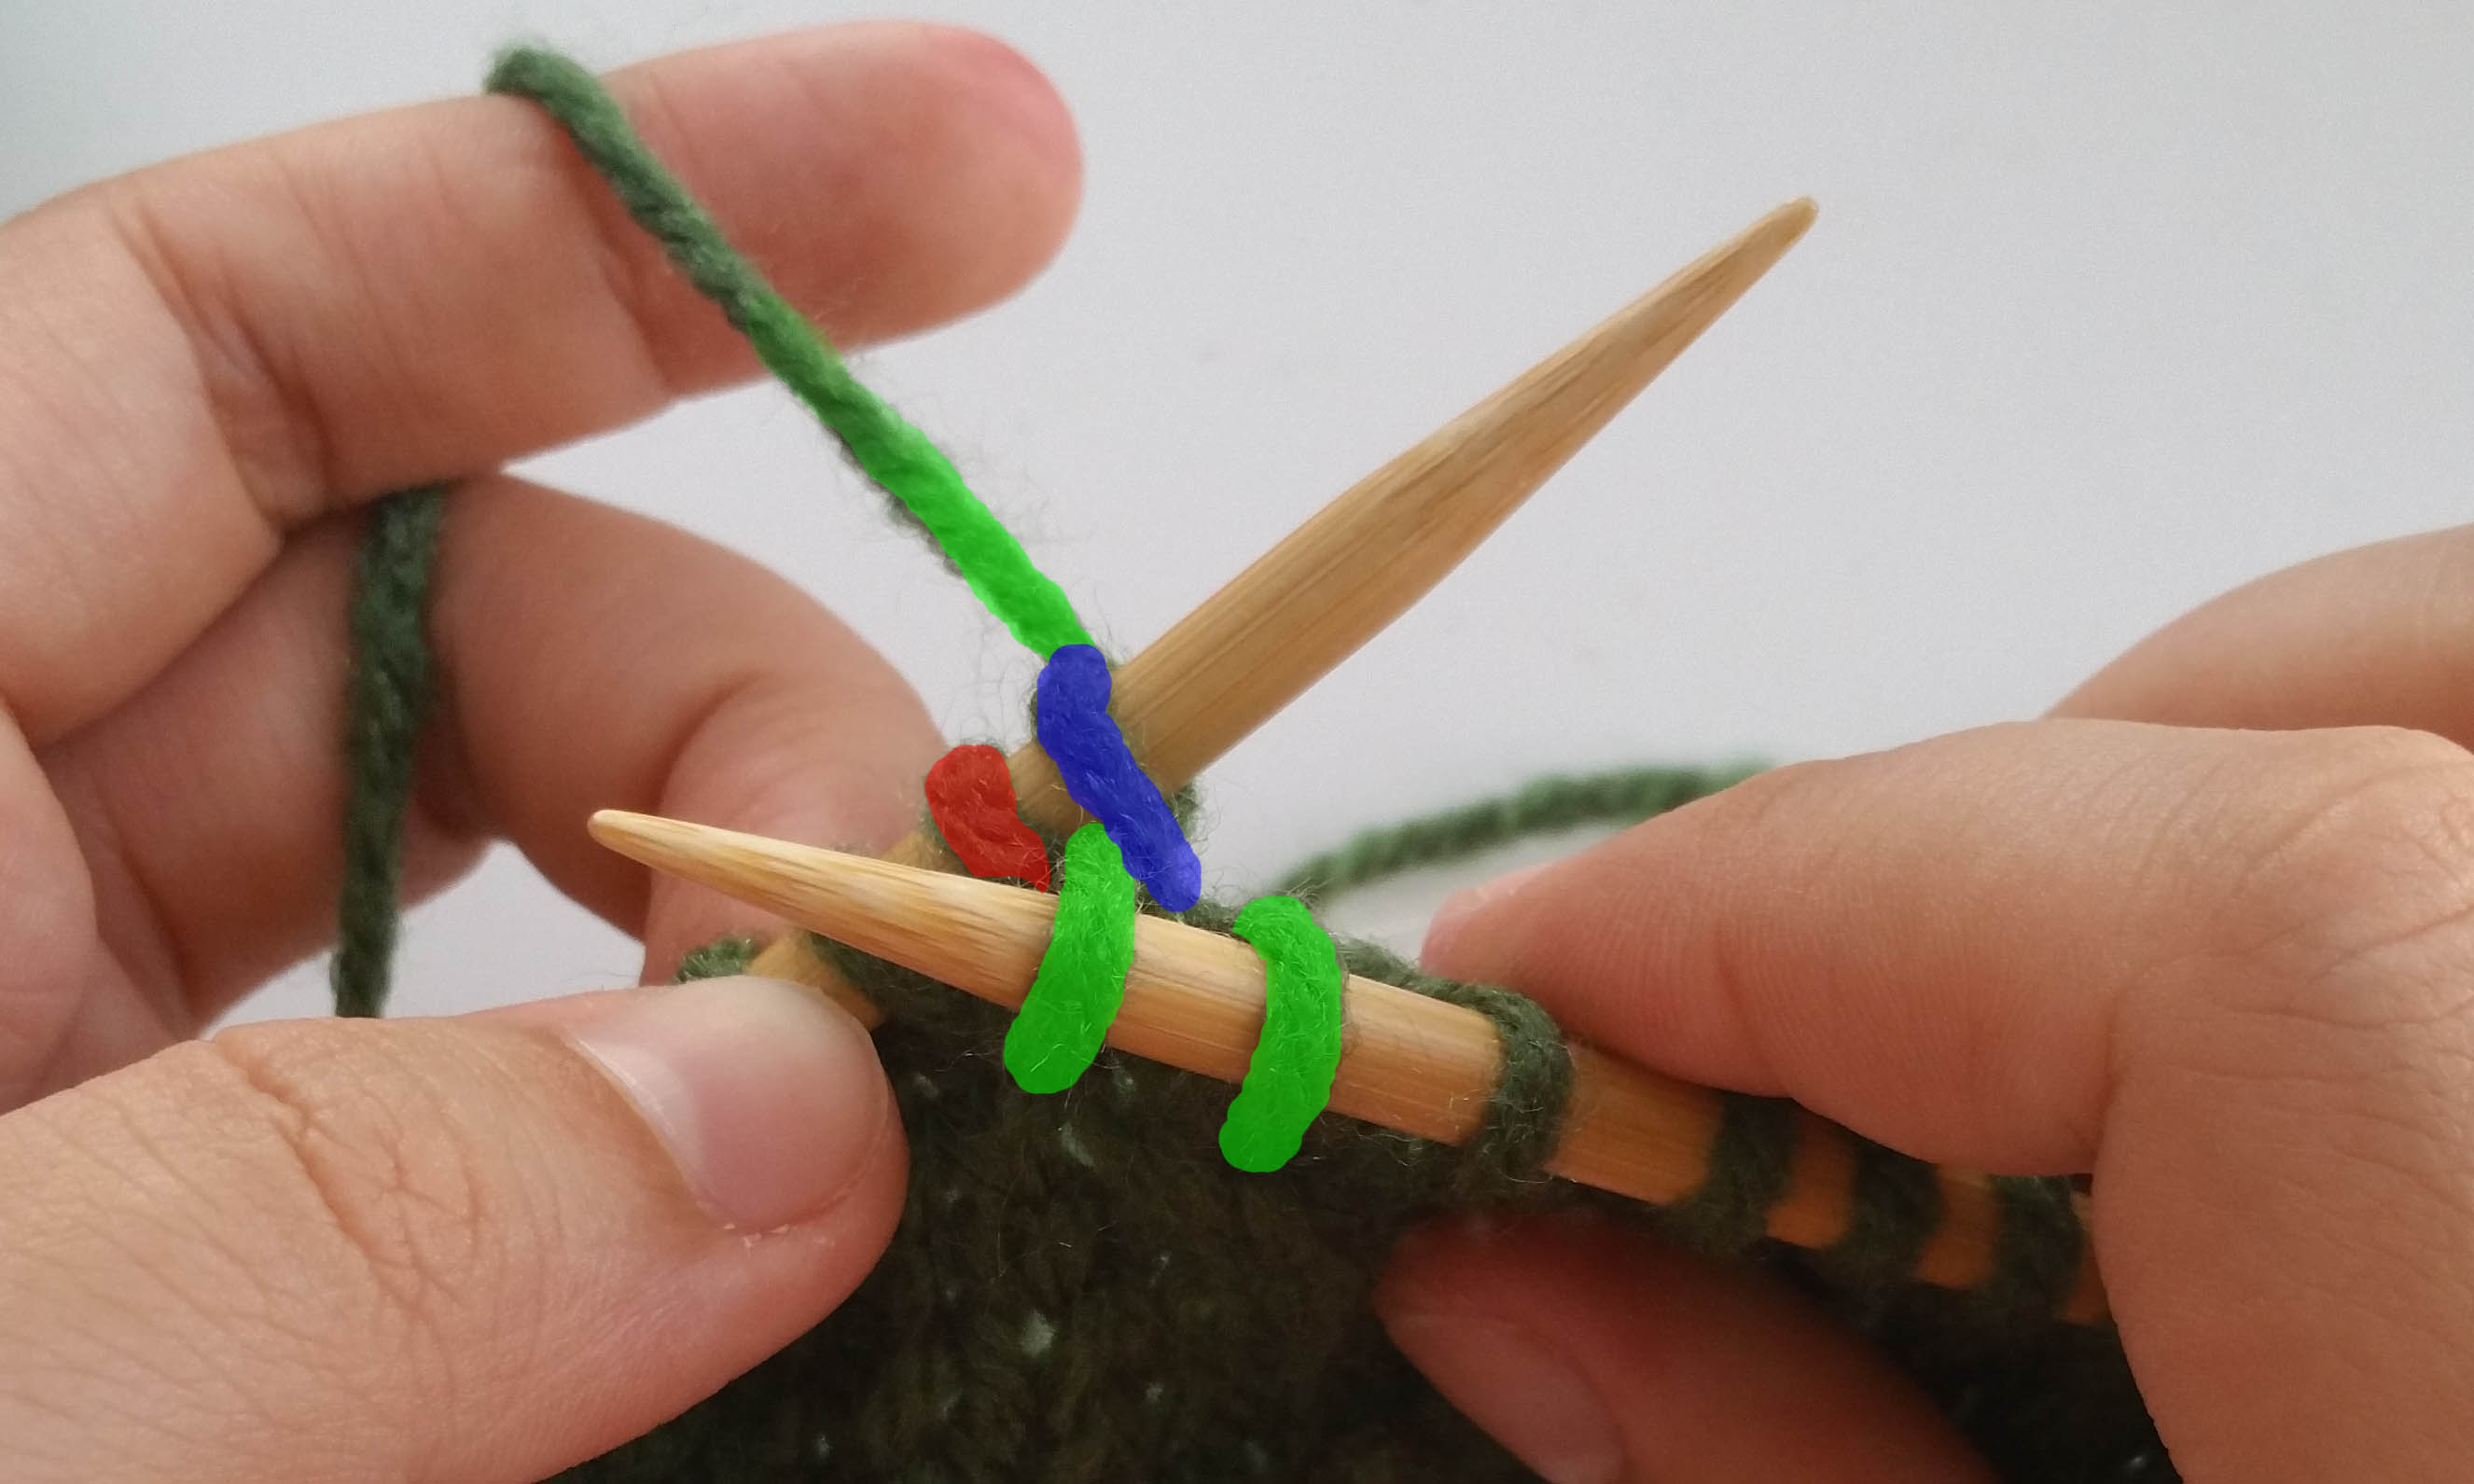
\includegraphics[width=2.5in]{rt_step5.jpg}

\item Drop both stitches off the left needle.

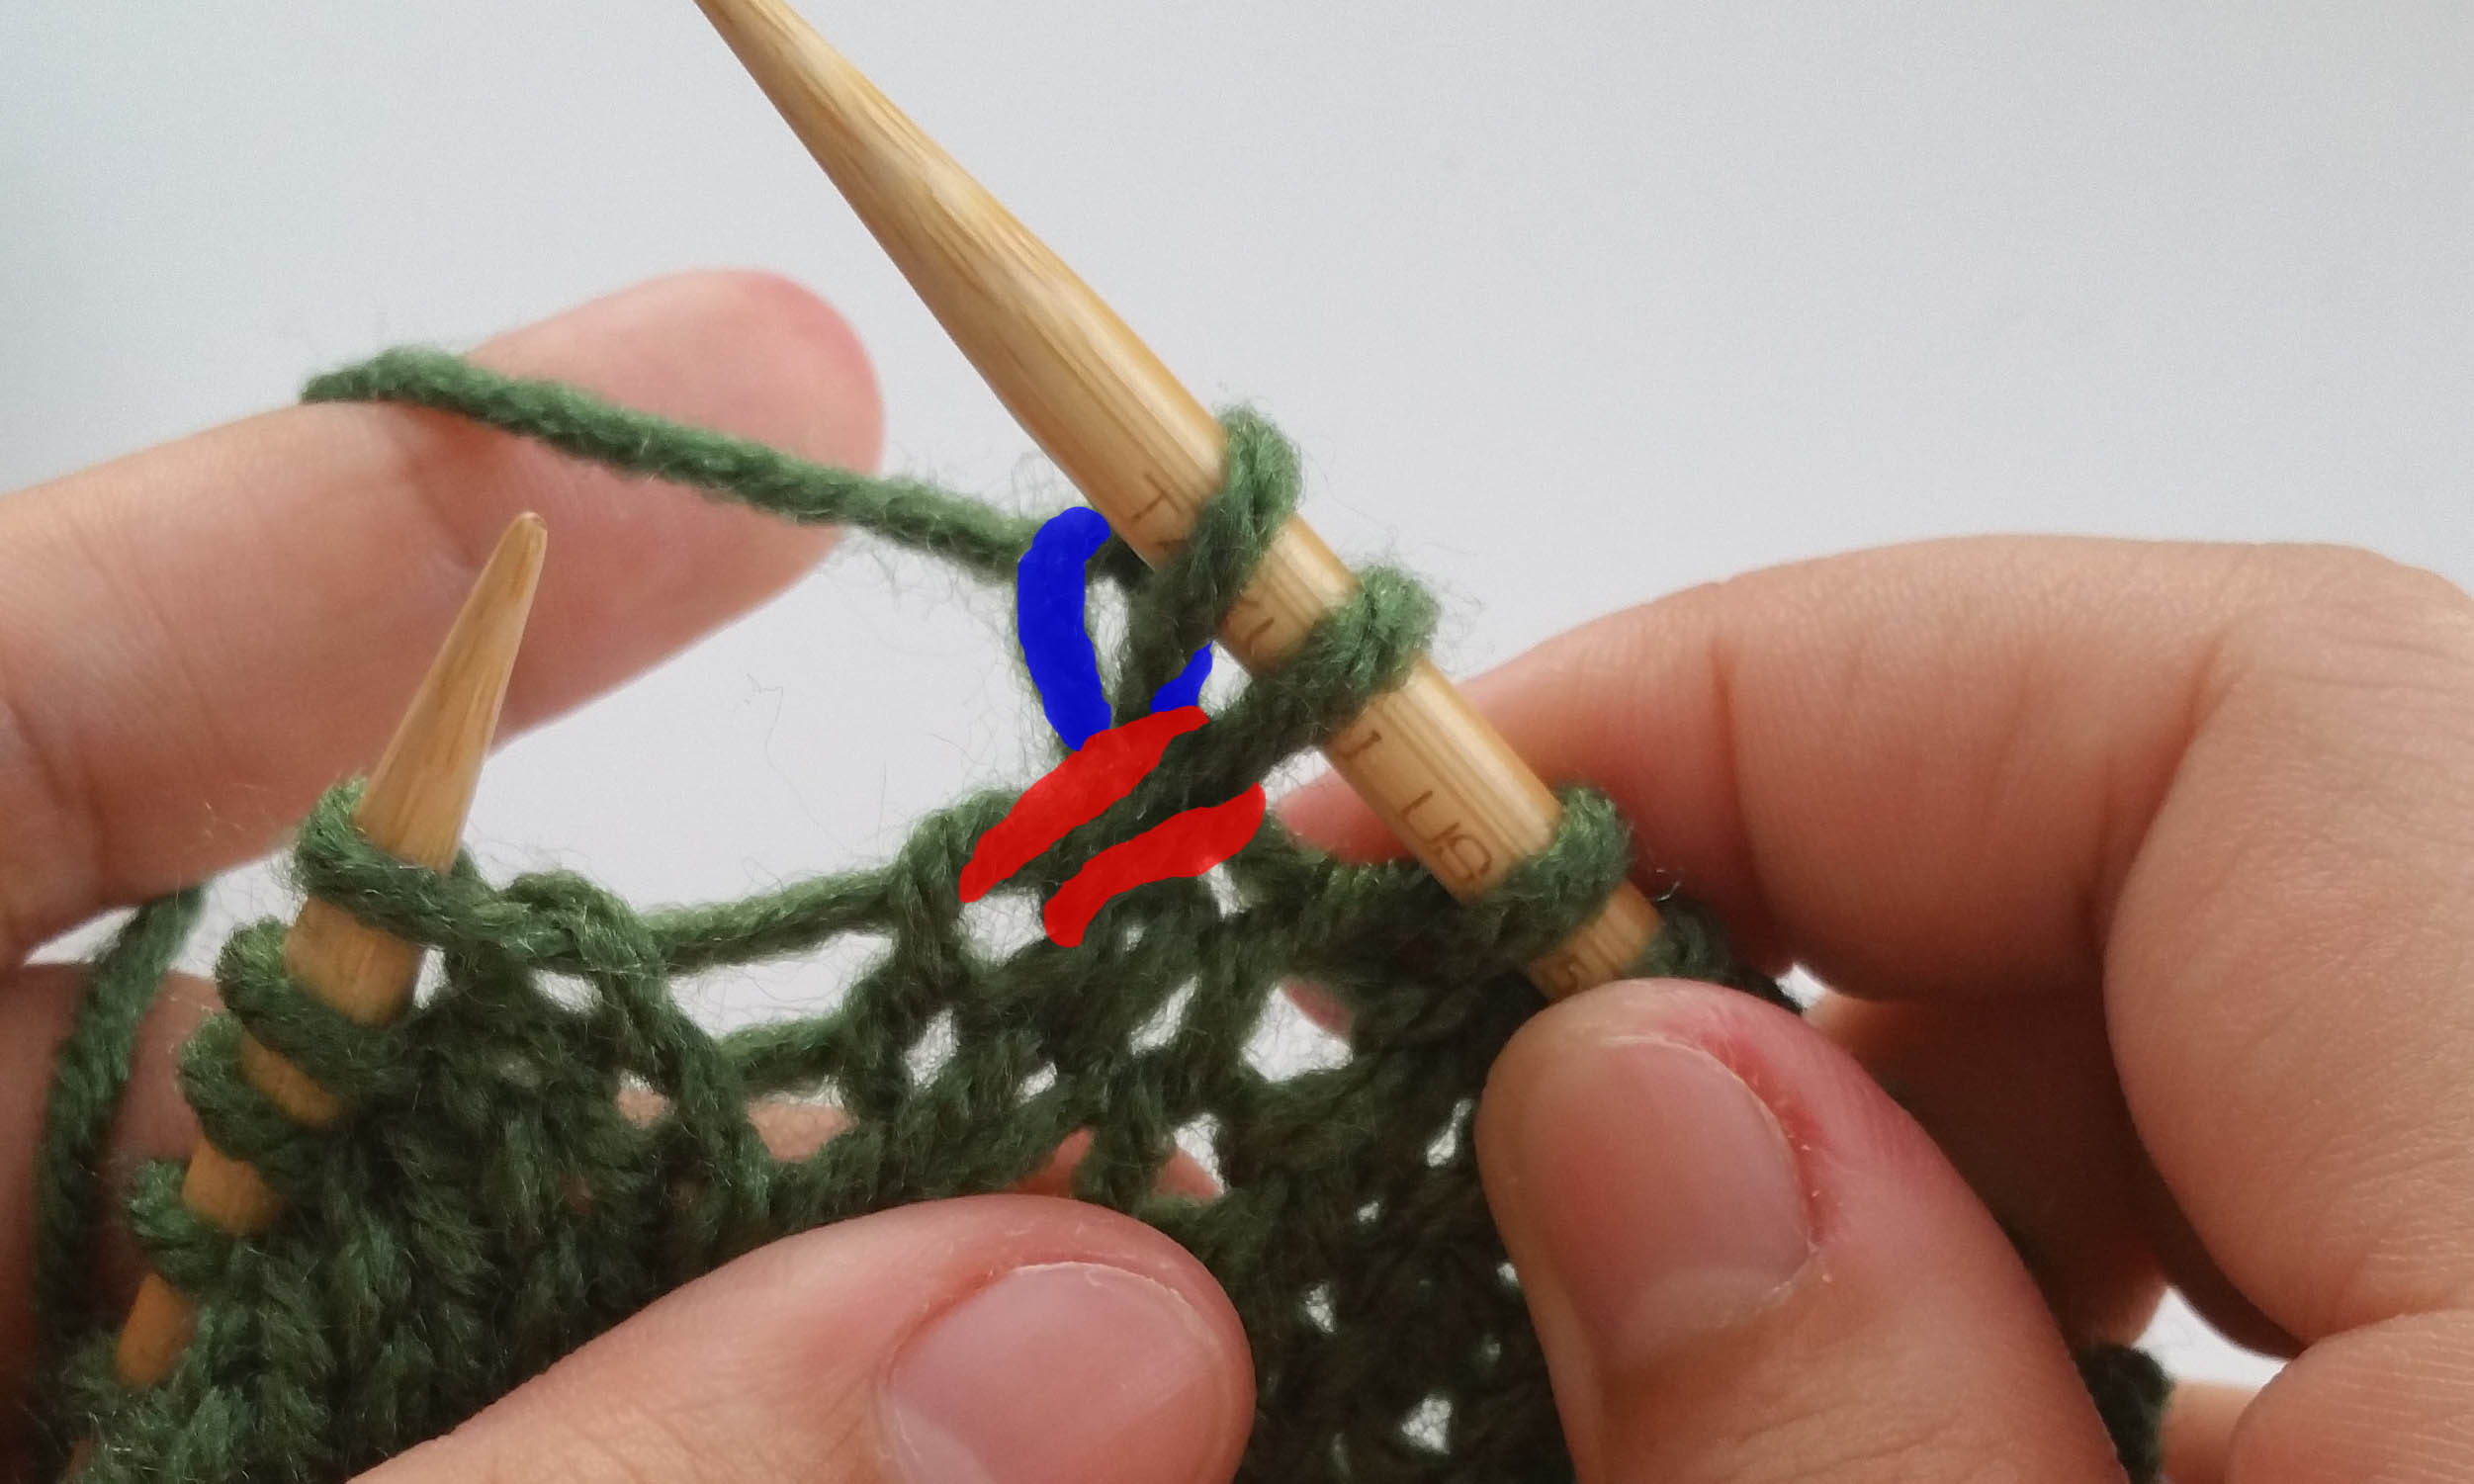
\includegraphics[width=2.5in]{rt_step6.jpg}

\end{enumerate}
\end{multicols}



\newpage
\section*{Appendix C: Tips for Modification}

I've included some tips for adapting this shawl for different yardages or desired sizes. Mitered Nova is structured in 7 sections, most of which can be shortened or extended by modifying the number of repeats in the section.

\vspace{1em}
To help you out with the math, I've included a table below with possible combinations of section sizes. In each section's column, the left number is the number of repeats of the section to work, while the right number is the resulting stitch count at the end of the section. Fill in the last section of the table with your chosen modifications ($a$, $b$, $c$, and $d$ for the number of section repeats). Your numbers must satisfy the equation \spine{$a + 5b = c + 2d$} in order for the stitch counts to work.
\vspace{-1em}
\begin{center}
\begin{tabular}{| L{0.2\linewidth} >{\columncolor{shadecolor}}C{0.05\linewidth}  C{0.1\linewidth} >{\columncolor{shadecolor}} C{0.05\linewidth}  C{0.1\linewidth} >{\columncolor{shadecolor}} C{0.05\linewidth}  C{0.1\linewidth} >{\columncolor{shadecolor}} C{0.05\linewidth}  C{0.1\linewidth} |} \thickhline
\multicolumn{9}{|l|}{\textbf{lace weight version} -  CO: 91 sts} \\ [-10pt]
{} 	& \multicolumn{2}{c}{Section 2}	&  \multicolumn{2}{c}{Section 3} 	& \multicolumn{2}{c}{Section 4} 	& \multicolumn{2}{ c |}{Section 5} \\ [-4pt]
sample \& written	& 30 & 121 sts & 8 & 161 sts & 40 & 121 sts & 15 & 91 sts \\ 
smaller shawl	& 25 & 116 sts & 8 & 156 sts & 35 & 121 sts & 15 & 91 sts \\ 
larger	shawl & 35 & 126 sts & 10 & 176 sts & 45 & 131 sts & 20 & 91 sts \\ 
more stripes & 35 & 126 sts & 5 & 151 sts & 10 & 141 sts & 25 & 91 sts \\ \thickhline
\multicolumn{9}{|l|}{\textbf{fingering weight} - CO: 71 sts} \\ [-10pt]
{} 	& \multicolumn{2}{c}{Section 2}	&  \multicolumn{2}{c}{Section 3} 	& \multicolumn{2}{c}{Section 4} 	& \multicolumn{2}{ c |}{Section 5} \\ [-4pt]
written	& 20 & 91 sts & 8 & 131 sts & 30 & 101 sts & 15 & 71 sts \\
sample (larger)	& 25 & 96 sts & 10 & 146 sts & 45 & 101 sts & 15 & 71 sts \\ 
smaller shawl	& 15 & 86 sts & 7 & 131 sts & 30 & 101 sts & 15 & 71 sts \\ 
more stripes	& 30 & 101 sts & 5 & 126 sts & 11 & 125 sts & 27 & 71 sts \\ \thickhline
\multicolumn{9}{|l|}{\textbf{your modified shawl} - CO: \underline{\hspace{40pt}}  sts} \\ [-10pt]
{} 	& \multicolumn{2}{c}{Section 2}	&  \multicolumn{2}{c}{Section 3} 	& \multicolumn{2}{c}{Section 4} 	& \multicolumn{2}{ c |}{Section 5} \\ [-4pt]
{}	& {$a$:\underline{\hspace{12pt}}} & {\underline{\hspace{25pt}} sts} & {$b$:\underline{\hspace{12pt}}} & {\underline{\hspace{25pt}} sts} & {$c$:\underline{\hspace{12pt}}} & {\underline{\hspace{25pt}} sts} & {$d$:\underline{\hspace{12pt}}} & {\underline{\hspace{25pt}} sts} \\ \thickhline
\end{tabular}
\end{center}

\vspace{1em}
In the following lists, I've outlined the some effects on the required yardage (C1 and C2) and on the mathematics of each section. Sections 2 and 3 both increase the number of stitches on your needles, while Sections 4 and 5 decrease the stitch count. Hence, any change in the size of the increase sections will \emph{require} changing the decrease sections. 

\newpage
\subsection*{Section 1}
\begin{itemize}
\item Section 1 does not increase or decrease the stitch count (hence the name ``steady state"), so the number of repeats may be modified to any arbitrary number. Your stitch count at the end of Section 1 should be the same as the stitch count at CO, 91 (71) sts.
\item If you have a shorter skein of C1, you may wish to work fewer repeats in Section 1.
\end{itemize}

\subsection*{Section 2}
\begin{itemize}
\item If you change the number of stripes in Section 2, make sure the number of \vocab{increase stripe} repeats is a multiple of 5 so that your stitch count at the end of Section 2 is a multiple of 5 plus 1 extra $[5n+1]$.
\end{itemize}

\subsection*{Section 3}
\begin{itemize}
\item Section 3 is where the stitch count changes most rapidly, so any change to the number of lace repeats will have a significant effect on the required amounts of C1 and C2.
\item Your final stitch count at the end of Section 3 should be a multiple of 5 plus 1 extra $[5n+1]$.
\end{itemize}

\subsection*{Section 4}
\begin{itemize}
\item Section 4 can eat up a lot of yardage from C1, so if you are concerned about running out of C1, work fewer repeats in this section. 

\item Your modifications for Section 4 will depend on how many stitches you had at the end of Section 3. After finishing Section 3, take your stitch count and subtract the original stitch count, 91 (71) sts, from it. If the difference is \vocab{even}, then work an even number of \vocab{decrease ridge} repeats in Section 4. If the difference is \vocab{odd}, then work an odd number of repeats in Section 4. This will ensure that you have an even number of stitches to decrease in Section 5.
\end{itemize}

\subsection*{Section 5}
\begin{itemize}
\item The ultimate goal of Section 5 is to decrease the stitch count until it is at the original number of stitches. Since each \vocab{decrease stripe} repeat in Section 5 decreases the total stitch count by 2 sts, you want to make sure that the difference between your stitch count at the beginning of the section and the original stitch count is \vocab{even}.
\end{itemize}

\subsection*{Section 6}
\begin{itemize}
\item Like Section 1, Section 6 does not change the number of stitches on your needles. It is also the last section in which you'll need C2, so you can work as many repeats as desired in order to use up C2.
\end{itemize}


\end{document}